%Version 3 December 2023
% See section 11 of the User Manual for version history
%
%%%%%%%%%%%%%%%%%%%%%%%%%%%%%%%%%%%%%%%%%%%%%%%%%%%%%%%%%%%%%%%%%%%%%%
%%                                                                 %%
%% Please do not use \input{...} to include other tex files.       %%
%% Submit your LaTeX manuscript as one .tex document.              %%
%%                                                                 %%
%% All additional figures and files should be attached             %%
%% separately and not embedded in the \TeX\ document itself.       %%
%%                                                                 %%
%%%%%%%%%%%%%%%%%%%%%%%%%%%%%%%%%%%%%%%%%%%%%%%%%%%%%%%%%%%%%%%%%%%%%

%%\documentclass[referee,sn-basic]{sn-jnl}% referee option is meant for double line spacing

%%=======================================================%%
%% to print line numbers in the margin use lineno option %%
%%=======================================================%%

%%\documentclass[lineno,sn-basic]{sn-jnl}% Basic Springer Nature Reference Style/Chemistry Reference Style

%%======================================================%%
%% to compile with pdflatex/xelatex use pdflatex option %%
%%======================================================%%

%%\documentclass[pdflatex,sn-basic]{sn-jnl}% Basic Springer Nature Reference Style/Chemistry Reference Style


%%Note: the following reference styles support Namedate and Numbered referencing. By default the style follows the most common style. To switch between the options you can add or remove “Numbered” in the optional parenthesis. 
%%The option is available for: sn-basic.bst, sn-vancouver.bst, sn-chicago.bst%  
 
%%\documentclass[pdflatex,sn-nature]{sn-jnl}% Style for submissions to Nature Portfolio journals
%%\documentclass[pdflatex,sn-basic]{sn-jnl}% Basic Springer Nature Reference Style/Chemistry Reference Style
\documentclass[pdflatex,sn-mathphys-num]{sn-jnl}% Math and Physical Sciences Numbered Reference Style 
%%\documentclass[pdflatex,sn-mathphys-ay]{sn-jnl}% Math and Physical Sciences Author Year Reference Style
%%\documentclass[pdflatex,sn-aps]{sn-jnl}% American Physical Society (APS) Reference Style
%%\documentclass[pdflatex,sn-vancouver,Numbered]{sn-jnl}% Vancouver Reference Style
%%\documentclass[pdflatex,sn-apa]{sn-jnl}% APA Reference Style 
%%\documentclass[pdflatex,sn-chicago]{sn-jnl}% Chicago-based Humanities Reference Style

%%%% Standard Packages
%%<additional latex packages if required can be included here>

\usepackage{graphicx}%
\usepackage{multirow}%
\usepackage{amsmath,amssymb,amsfonts}%
\usepackage{amsthm}%
\usepackage{mathrsfs}%
\usepackage[title]{appendix}%
\usepackage{xcolor}%
\usepackage{textcomp}%
\usepackage{manyfoot}%
\usepackage{booktabs}%
\usepackage{algorithm}%
\usepackage{algorithmicx}%
\usepackage{algpseudocode}%
\usepackage{listings}%

%% For algorithms...
\algnewcommand\algorithmicforeach{\textbf{for each}}
\algdef{S}[FOR]{ForEach}[1]{\algorithmicforeach\ #1\ \algorithmicdo}
\algnewcommand\algorithmicswitch{\textbf{switch}}
\algnewcommand\algorithmiccase{\textbf{case}}
\algdef{SE}[SWITCH]{Switch}{EndSwitch}[1]{\algorithmicswitch\ #1\ \algorithmicdo}{\algorithmicend\ \algorithmicswitch}
\algdef{SE}[CASE]{Case}{EndCase}[1]{\algorithmiccase\ #1}{\algorithmicend\ \algorithmiccase}
\algtext*{EndSwitch}
\algtext*{EndCase}
%%%%

%%%%%=============================================================================%%%%
%%%%  Remarks: This template is provided to aid authors with the preparation
%%%%  of original research articles intended for submission to journals published 
%%%%  by Springer Nature. The guidance has been prepared in partnership with 
%%%%  production teams to conform to Springer Nature technical requirements. 
%%%%  Editorial and presentation requirements differ among journal portfolios and 
%%%%  research disciplines. You may find sections in this template are irrelevant 
%%%%  to your work and are empowered to omit any such section if allowed by the 
%%%%  journal you intend to submit to. The submission guidelines and policies 
%%%%  of the journal take precedence. A detailed User Manual is available in the 
%%%%  template package for technical guidance.
%%%%%=============================================================================%%%%

%% as per the requirement new theorem styles can be included as shown below
%\theoremstyle{thmstyleone}%
\newtheorem{theorem}{Theorem}%  meant for continuous numbers
%%\newtheorem{theorem}{Theorem}[section]% meant for sectionwise numbers
%% optional argument [theorem] produces theorem numbering sequence instead of independent numbers for Proposition
\newtheorem{proposition}[theorem]{Proposition}% 
%%\newtheorem{proposition}{Proposition}% to get separate numbers for theorem and proposition etc.

%\theoremstyle{thmstyletwo}%
\newtheorem{example}{Example}%
\newtheorem{remark}{Remark}%

%\theoremstyle{thmstylethree}%
\newtheorem{definition}{Definition}%
\newtheorem{lemma}{Lemma}


\raggedbottom
%%\unnumbered% uncomment this for unnumbered level heads

\begin{document}

\title[SDCEL]{On Scalable DCEL Overlay Operations}

%%=============================================================%%
%% GivenName	-> \fnm{Joergen W.}
%% Particle	-> \spfx{van der} -> surname prefix
%% FamilyName	-> \sur{Ploeg}
%% Suffix	-> \sfx{IV}
%% \author*[1,2]{\fnm{Joergen W.} \spfx{van der} \sur{Ploeg} 
%%  \sfx{IV}}\email{iauthor@gmail.com}
%%=============================================================%%

\author*[1]{\fnm{Andres} \sur{Calderon-Romero}}\email{acald013@ucr.edu}

\author[1]{\fnm{Laila} \sur{Abdelhafeez}}\email{labde005@ucr.edu}

\author[2]{\fnm{Goce} \sur{Trajcevski}}\email{gocet25@iastate.edu}

\author[1]{\fnm{Amr} \sur{Magdy}}\email{amr@cs.ucr.edu}

\author[1]{\fnm{Vassilis J.} \sur{Tsotras}}\email{tsotras@cs.ucr.edu}

\affil[1]{\orgdiv{Computer Science Department}, \orgname{University of California}, \orgaddress{\street{900 University Ave}, \city{Riverside}, \postcode{92521}, \state{California}, \country{US}}}
\affil[2]{\orgdiv{Department of Electrical and Computer Engineering}, \orgname{Iowa State University}, \orgaddress{\street{2433 Union Dr}, \city{Ames}, \postcode{50011}, \state{Iowa}, \country{US}}}

%%==================================%%
%% Sample for unstructured abstract %%
%%==================================%%

\abstract{
The Doubly Connected Edge List (DCEL) is an edge-list structure widely used in spatial applications, primarily for planar topological and geometric computations. However, it is also applicable to various types of data, including 3D models and geographic data.
An essential operation is the \textit{overlay operation}, which combines the DCELs of two input polygon layers and can easily support spatial queries on polygons like the intersection, union, and difference between these layers.
However, existing techniques for spatial overlay operations suffer from two main limitations.
First, they fail to handle many large datasets practically used in real applications.
Second, they cannot handle arbitrary spatial lines that practically form polygons, e.g., city blocks, but they are given as a set of scattered lines.
This work proposes a distributed and scalable way to compute the overlay operation and its related supported queries. Our operations also support arbitrary spatial lines through a scalable polygonization process.
We address the issues of efficiently distributing the lines and overlay operators and offer various optimizations that improve performance. Our experiments demonstrate that the proposed scalable solution can efficiently compute the overlay of large real datasets.}

%%================================%%
%% Sample for structured abstract %%
%%================================%%

% \abstract{\textbf{Purpose:} The abstract serves both as a general introduction to the topic and as a brief, non-technical summary of the main results and their implications. The abstract must not include subheadings (unless expressly permitted in the journal's Instructions to Authors), equations or citations. As a guide the abstract should not exceed 200 words. Most journals do not set a hard limit however authors are advised to check the author instructions for the journal they are submitting to.
% 
% \textbf{Methods:} The abstract serves both as a general introduction to the topic and as a brief, non-technical summary of the main results and their implications. The abstract must not include subheadings (unless expressly permitted in the journal's Instructions to Authors), equations or citations. As a guide the abstract should not exceed 200 words. Most journals do not set a hard limit however authors are advised to check the author instructions for the journal they are submitting to.
% 
% \textbf{Results:} The abstract serves both as a general introduction to the topic and as a brief, non-technical summary of the main results and their implications. The abstract must not include subheadings (unless expressly permitted in the journal's Instructions to Authors), equations or citations. As a guide the abstract should not exceed 200 words. Most journals do not set a hard limit however authors are advised to check the author instructions for the journal they are submitting to.
% 
% \textbf{Conclusion:} The abstract serves both as a general introduction to the topic and as a brief, non-technical summary of the main results and their implications. The abstract must not include subheadings (unless expressly permitted in the journal's Instructions to Authors), equations or citations. As a guide the abstract should not exceed 200 words. Most journals do not set a hard limit however authors are advised to check the author instructions for the journal they are submitting to.}

\keywords{Spatial data structures, overlay operator, DCEL}

%%\pacs[JEL Classification]{D8, H51}

%%\pacs[MSC Classification]{35A01, 65L10, 65L12, 65L20, 65L70}

\maketitle

\section{Introduction} %\label{sec:extenstion_introduction}

This chapter extends the previous work in \cite{calderon_scalable_2023}. The main new contributions are summarized as follows. First, we introduce a new spatial partitioner, based on the kd-tree partitioning strategy, for constructing overlay  DCELs (section \ref{sec:pstrategies}). Since it better utilizes the data distributions in optimizing DCEL partitions, it leads to noticeably improved performance. The new partitioning strategy contrasts with the original strategy that employed space-partitioning techniques based on quadtrees. 

Second, we extend the overlay DCEL approach to accept scattered and noisy line segments as input, rather than being restricted to clean polygon data. This enhancement builds on the scalable polygonization methods presented in \cite{abdelhafeez_ddcel_2023}, enabling the overlay of real-world datasets composed of vast sets of line segments —datasets that existing techniques are unable to process effectively.

For instance, Figure \ref{fig:extension_dcel_example} illustrates the fundamental components of a DCEL. Additionally, we identify two types of special half-edges. \textit{Dangles} are half-edges with one or both endpoints not incident on another half-edge endpoint; both half-edge $\overrightarrow{fj}$ and its twin are considered dangle edges. \textit{Cut-edges} are half-edges connected at both ends that do not form part of any polygon. The half-edge $\overrightarrow{dg}$ and its twin are classified as cut-edges.

\begin{figure}
    \centering
    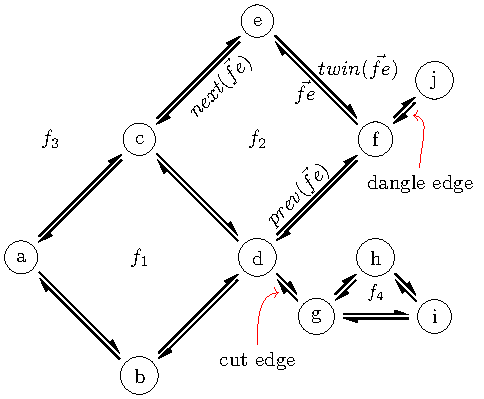
\includegraphics[width=0.6\linewidth]{chapterExtension/dcel_example2}
    \caption{Components of the DCEL structure with dangle and cut edges.}\label{fig:extension_dcel_example}
\end{figure}

The remainder of this chapter is organized as follows. Section \ref{sec:extension_methods} details the implementation of the new kd-tree partitioner and describes the polygon extraction process for adapting line segment inputs, which extends the overlay method to support dangle and cut edges. In Section \ref{sec:extension_experiments}, we present additional experiments to quantify the benefits of the kd-tree-based strategy and assess the performance of the proposed polygonization on datasets with large volumes of line segments.

\section{Related Work}\label{sec:related}
The fundamentals of the DCEL data structure were introduced in the seminal paper by Muller and Preparata  \cite{muller_finding_1978}. The advantages of DCELs are highlighted in \cite{preparata_computational_1985, berg_computational_2008}. Examples of using DCELs for diverse applications appear in \cite{barequet_dcel_1998, boltcheva_topological-based_2020, freiseisen_colored_1998}.

Once the overlay DCEL is created by combining two layers, overlay operators like union, difference, etc., can be computed in linear time to the number of faces in their overlay \cite{freiseisen_colored_1998}. 
Currently, few sequential implementations are available: LEDA \cite{mehlhorn_leda_1995}, Holmes3D
\cite{holmes_dcel_2021} and CGAL \cite{fogel_cgal_2012}. Among them, CGAL is an open-source project widely used for computational geometry research. To the best of our knowledge, there is no scalable implementation for the computation of DCEL overlay.

While there is a lot of work on using spatial access methods to support spatial joins, intersections, unions etc. in a parallel way (using clusters, multicores or GPUs), \cite{challa_dd-rtree_2016, sabek_spatial_2017, li_scalable_2019, franklin_data_2018, magalhaes_fast_2015, puri_efficient_2013, puri_mapreduce_2013} these approaches are different in two ways: (i) after the index filtering, they need a time-consuming refine phase where the operator (union, intersection etc.) has to be applied on each pair of (typically) complex spatial objects; (ii) if the operator changes, we need to run the filter/refine phases from scratch (in contrast, the same overlay DCEL can be used to run all operators.)

\section{Scalable Kd-tree Partitioner with Dangle and Cut Edges Integration} \label{sec:extension_methods}

\subsubsection{Kd-tree Partition Strategy} %\label{sec:kdtreestrategy}
In Section \ref{sec:pstrategies}, we use the quadtree spatial index as the baseline for our partitioning strategy. The quadtree follows a space-oriented approach, as it does not consider the content of each cell when determining potential splits. In contrast, kd-tree-based partitioning employs a data-oriented approach by sorting and selecting the midpoint within a cell to guide the placement of splits for future child nodes.

Building and populating the kd-tree partitioning follows a process similar to that of the quadtree. First, a kd-tree is constructed from a sample representing 1\% of the input data to define the tree’s structure, where the leaves represent the partition’s cells. The input data is then fed into this kd-tree structure, with each edge assigned to the leaf cell containing its boundaries. After partitioning, the local DCELs for each layer are constructed, and the overlay operation is performed within each cell as described in Section \ref{sec:pstrategies}.

Section \ref{sec:extension_experiments} will compare two partitioning strategies, the one presented in \ref{sec:pstrategies} based on the quadtree (i.e. space-oriented) and one on the kd-tree (i.e. data-oriented) indexes.  Note that both tree-based data partitioning involves shuffling all edges; this however, happens only once. Our experimental evaluation (see Section \ref{sec:comparison}) shows that the data-oriented approach leads to better performance. 

\subsection{Overlaying Polygons with Dangle and Cut Edges} \label{sec:over_dang}

Beyond scalability challenges, many modern applications receive spatial polygon datasets as scattered line segments—for example, road segments that form city blocks. Such datasets can be extremely large and are common in fields like urban planning, geo-targeted advertising, economic and demographic studies, and more. However, existing polygon overlay techniques are not equipped to process them directly at scale. In this section, we extend the overlay method presented in Section \ref{sec:methods} to support polygonal input by integrating a scalable, distributed polygon extraction approach. This enhancement enables the merging of polygons with dangle and cut edges.

We built on in the scalable polygonization procedure presented in \cite{abdelhafeez_ddcel_2023}.  The result of that polygonization procedure generates two outputs: first, a set of closed polygons formed by the input planar line segments, and second, any edges that are not a part of any polygon (i.e., dangle or cut edges).  Overlaying the polygons generated with any polygon layer follows the approaches discussed in sections \ref{sec:methods} and \ref{sec:alternative_methods}.  However, we need to modify the algorithms provided in these previous sections to overlay an input polygon layer $A$ with the dangle and cut edges (layer $B$). In particular, we modify the reduce phase.

We build upon the scalable polygonization procedure presented in \cite{abdelhafeez_ddcel_2023} (see Figure \ref{fig:polygonization}), which produces two outputs: (1) a set of closed polygons formed from the input planar line segments, and (2) any edges that are not part of any polygon (i.e., dangle or cut edges). Overlaying these generated polygons with any polygon layer follows the methods discussed in Sections \ref{sec:methods} and \ref{sec:alternative_methods}. However, to overlay an input polygon layer $A$ with the dangle and cut edges (layer $B$), we modify the algorithms from these sections, particularly adjusting the reduce phase.

 \begin{figure}
     \centering
     \begin{tabular}{cc}
         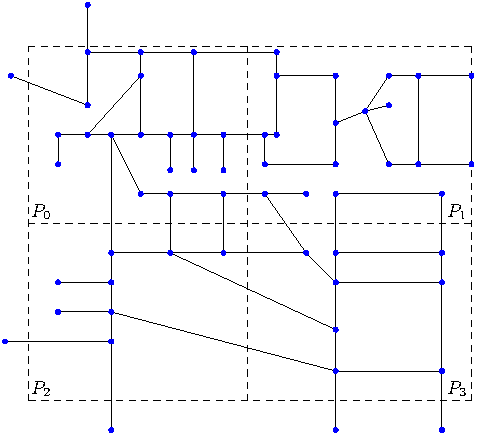
\includegraphics[width=0.49\textwidth]{chapterExtension/model/input/input} &
         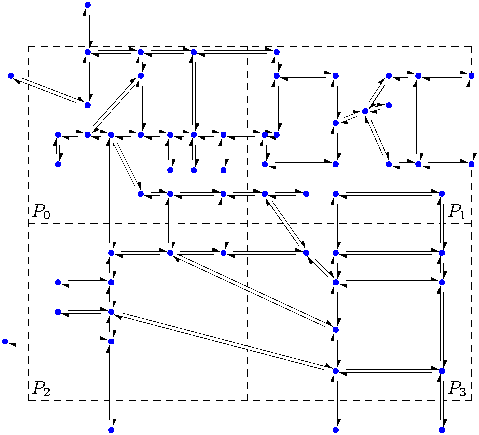
\includegraphics[width=0.49\textwidth]{chapterExtension/model/a/a} \\
         (a) & (b) \\
         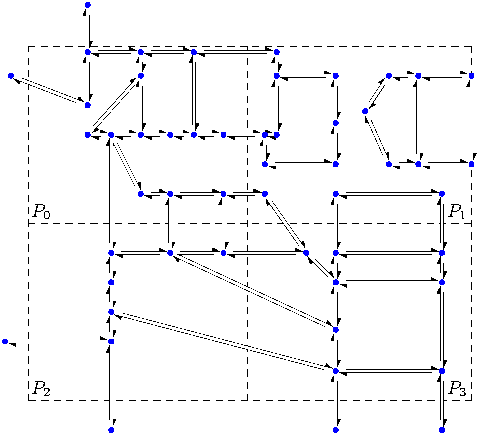
\includegraphics[width=0.49\textwidth]{chapterExtension/model/b/b} &
         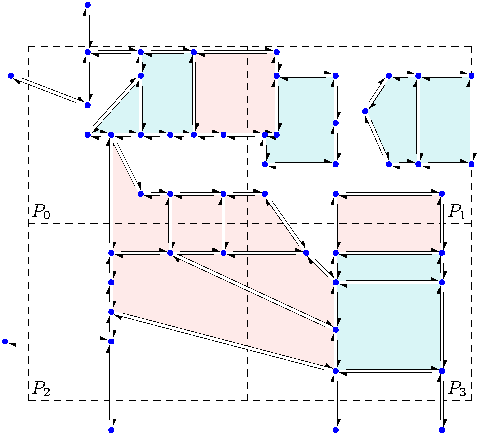
\includegraphics[width=0.49\textwidth]{chapterExtension/model/c/c} \\
         (c) & (d) \\
     \end{tabular}
     \caption{An example of four leaf nodes in a quadtree constructed for input spatial line segments. Solid lines represent the line segments, while dashed lines indicate the Minimum Bounding Rectangles (MBRs) of the partitions. (a) shows the partitioned input spatial lines. (b) shows the DCEL vertices and half-edges. (c) the resulting DCEL after  dangle and cut edge removal.  Finally, (d) shows the final DCEL faces. (taken from \cite{abdelhafeez_ddcel_2023}).} \label{fig:polygonization}
 \end{figure}

 \begin{figure}
    \centering
    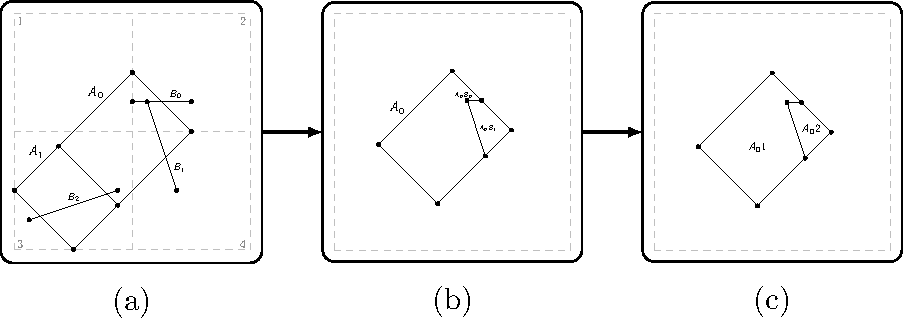
\includegraphics[width=\textwidth]{chapterExtension/dangles_cuts/DAC}
    \caption{(a) Spatial partitioning of input layers A and B, (b) Re-Partitioning of polygon $A_0$ with edges it intersects with, and (c) the result of polygonization of $A_0$ with $B_0, B_1, B_2$.} \label{fig:dangles_cuts}
 \end{figure}

 Figure \ref{fig:dangles_cuts}(a) illustrates the spatial partitioning of two input layers, $A$ and $B$. Layer $A$ contains two input polygons, $A_0$ and $A_1$, while Layer $B$ includes of three dangle edges, $B_0$, $B_1$, and $B_2$.
 
 Each edge in layer $B$ is assigned a unique label and provided as input to the overlay module.  The local overlay processs indentifies intersections between the input polygon layer $A$ and layer $B$ within each data partition.  If a polygon with $id = i$ from layer $A$ intersects with edges labeled $id = a$, $id = b$ and $id = c$ from layer $B$ in a given partition, a composite label $A_{i} B_{a} B_{b} B_{c}$ is generated to represent these intersections.  
 
During the reduce phase, we re-partition the data based on the first label, consolidating all edges that intersect with it. For instance, if two data partitions generate the labels $A_{i} B_{a} B_{b} B_{c}$ and $A_{i} B_{x} B_{y}$, we reassign the data so that $A_{i}$ is grouped within a single partition along with all intersecting edges, specifically $B_{a}, B_{b}, B_{c}, B_{x}, B_{y}$.  In Figure \ref{fig:dangles_cuts}(b), polygon $A_0$ is re-partitioned with the edges it intersects, namely $B_0$, $B_1$, and $B_2$.

After re-partitioning, all intersecting edges from both layers are consolidated within the same partition. The next step is to identify the polygons formed by these intersections. Since there is no guarantee that only one polygon will be generated, we replace the polygon concatenation method proposed in Section \ref{sec:optimizing} with a \textit{polygonization} procedure within each partition. This polygonization process ensures that all possible new polygons are generated.

The polygonization procedure follows the algorithm outlined in \cite{abdelhafeez_ddcel_2023}. It begins by generating new vertices and half-edges, marking the current dangle and cut edges, setting the next pointers, and finally constructing the partition polygons. Figure \ref{fig:dangles_cuts}(c) illustrates the result of polygonizing the edges from polygon$A_0$ and $B_0$, $B_1$, and $B_2$, yielding two polygons,$A_01$ and $A_02$.  The polygons generated from all partitions together form the overlay between polygon layer $A$ and layer $B$.

\section{Scalable Polygon Extraction for Line-based Input} \label{sec:polygonization}

Our discussion so far assumed the input data is a set of clean and closed polygons in the two input layers to be overlayed. However, several real-world 
polygons, such as city blocks formed by individual road segments represented as spatial lines, are unavailable in the polygonal form. Forming polygons in such 
cases at a large scale is non-trivial and takes significant computing cost. This section further extends our scalable DCEL overlay operations to handle 
scattered line segments as input through a scalable polygonization \cite{abdelhafeez_ddcel_2023} process. Such a feature enables spatial data scientists to 
seamlessly  
exploit a rich set of publicly available datasets, e.g., spatial road networks worldwide \cite{web:data:continents,web:data:usa}.

\begin{figure}[tb]
	\centering
	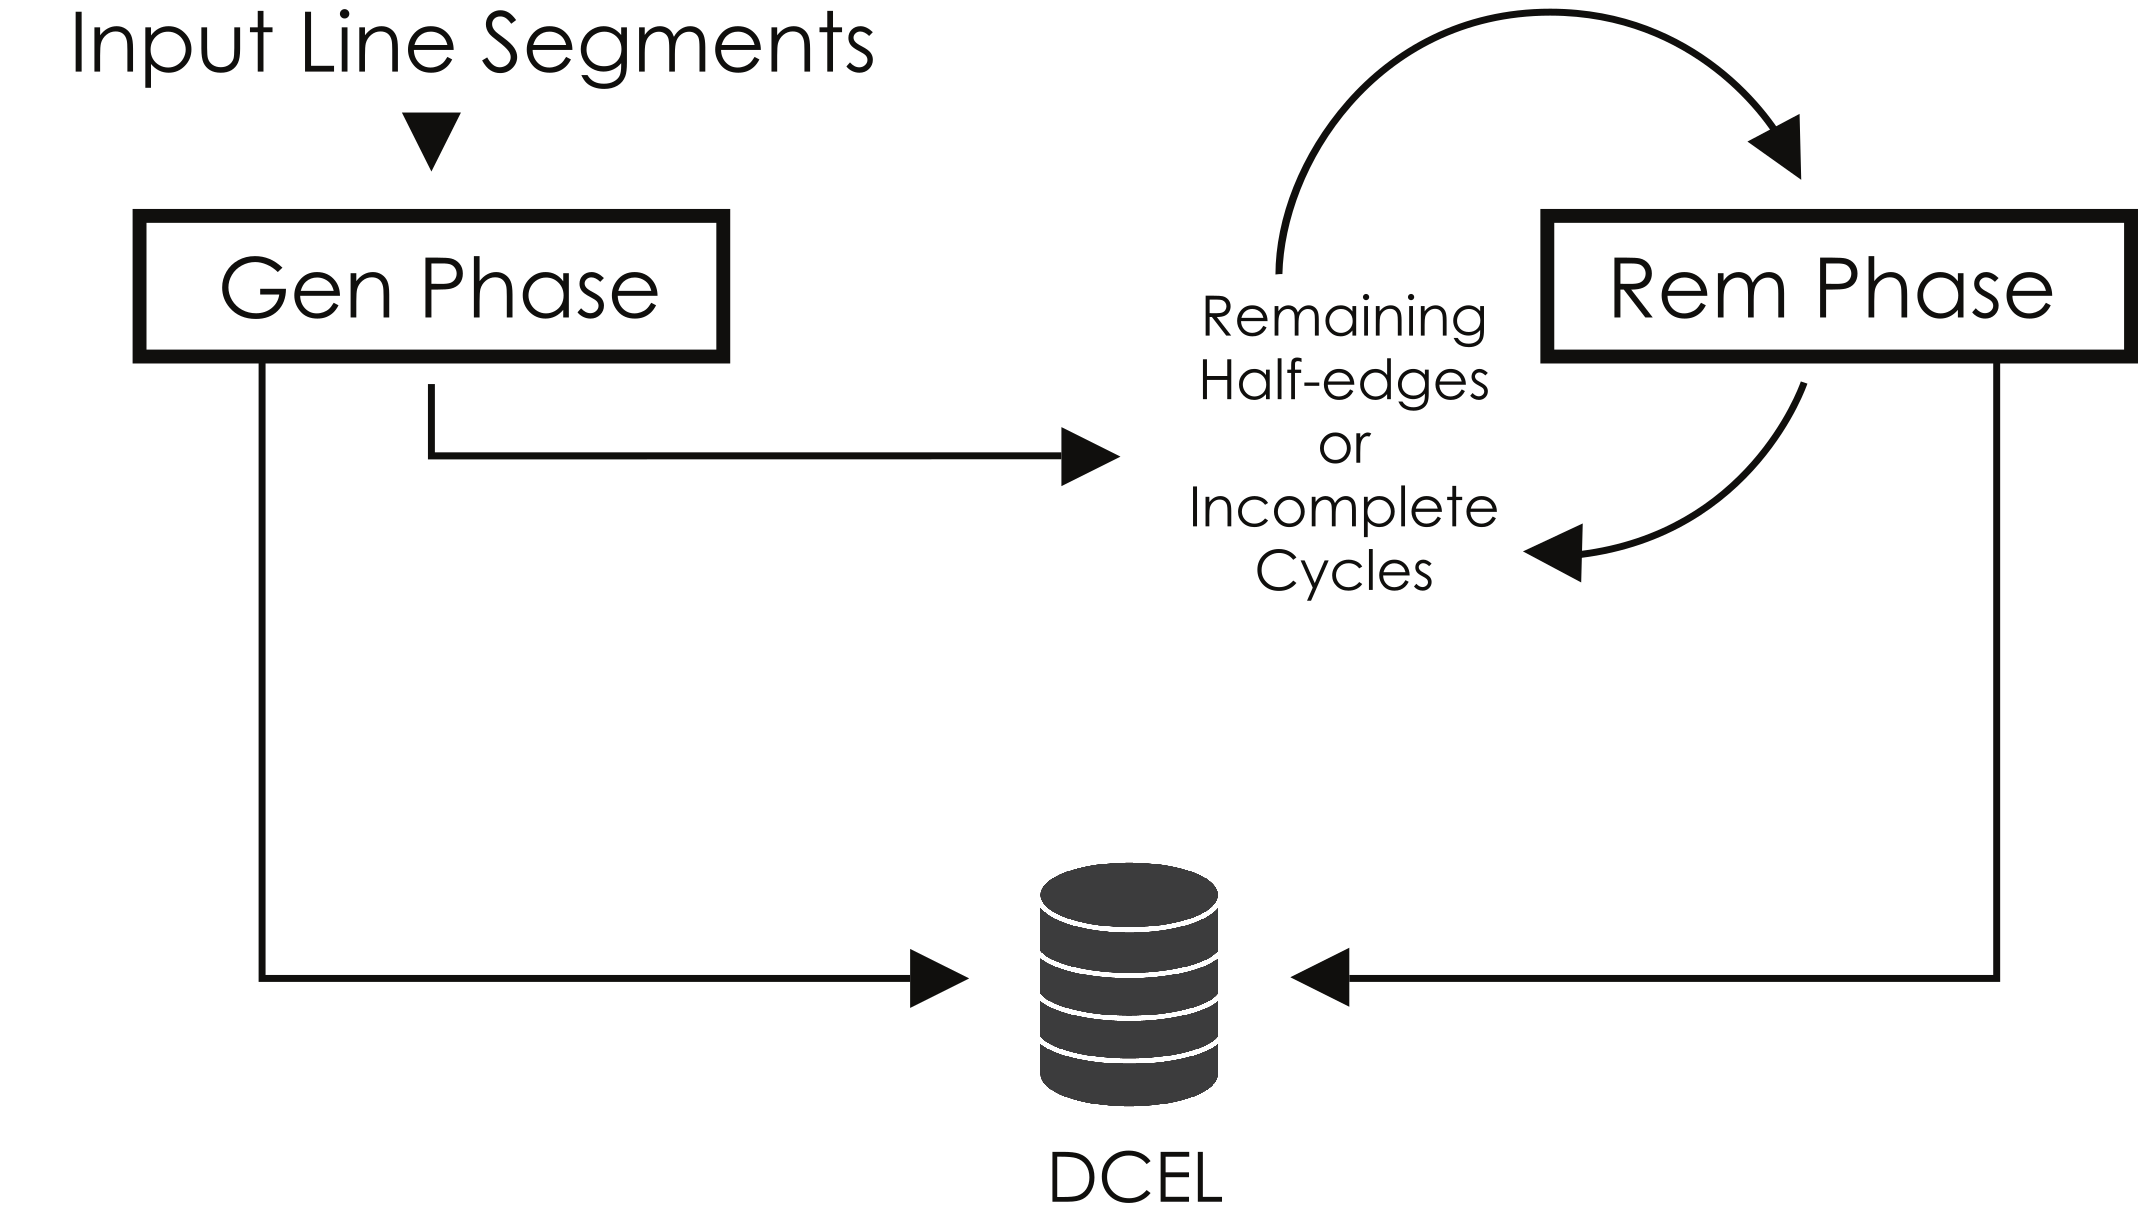
\includegraphics[width=0.75 \linewidth ]{chapterSDCEL/model/overview_updated.png}
	\caption{DCEL Constructor for Polygonization Overview}
	\label{fig:overview_ddcel}
\end{figure}

Building a DCEL data structure from an input of planar line segments extracts all closed polygons during the invocation of the \textit{polygonization} 
procedure.  In our work in \cite{abdelhafeez_ddcel_2023}, we proposed a scalable distributed framework to build a DCEL and extract polygons in parallel from 
the 
input 
line segments. Figure \ref{fig:overview_ddcel} shows an overview of the DCEL constructor. 

To create a DCEL data structure from input line segments, the \textit{DCEL constructor} undergoes a two-phase paradigm.  The \textit{Gen Phase}, detailed in 
Section \ref{sec:gen}, spatially partitions the input lines, generating the subdivision's vertices ($V$) and half-edges ($H$), and a subset of the 
subdivision's faces ($F_0$). 

The remaining line segments that are not assigned to a face yet are passed to the subsequent phase in the form of half-edges or incomplete cycles. An 
incomplete 
cycle is a connected half-edge list that is a candidate face. The \textit{Rem Phase}, detailed in Section \ref{sec:rem}, generates the subdivision's remaining 
faces, $F_j, \ \forall j > 0$. 

Section \ref{sec:partitioning_ddcel} discusses different data re-partitioning schemes with a minimal number of iterations to reduce the workload of the 
\textit{Rem Phase} without compromising correctness. The polygonization procedure produces two outputs: first, a set of closed polygons formed by the input 
planar line segments, and second, any edges that are not a part of any polygon, i.e., dangle or cut edges. Overlaying the polygons generated with any polygon 
layer follows the approaches discussed in sections \ref{sec:methods}and \ref{sec:alternative_methods}. In section \ref{sec:over_dang}, we extend the overlay 
approaches to handle overlaying a polygon layer with the remaining edges (the dangle and cut edges).

\subsection{Gen Phase}
\label{sec:gen}

The Gen phase accepts an input dataset of line segments $N$ and starts by partitioning the input across the worker nodes in a distributed cluster using a global quadtree spatial index.
Each data partition $P_i$ covers a specific spatial area represented by its minimum bounding rectangle (MBR) $B_i$.
Figure~\ref{fig:ddcel:input} shows an example of four leaf nodes of a quadtree built for input spatial line segments. Solid lines represent the line segments, and dashed lines represent the partitions' MBRs.

\begin{figure}[tb]
	\centering
	
\includegraphics[width=0.75 \linewidth ]{chapterSDCEL/model/input-network}
	\caption{Partitioned input spatial lines.}
	\label{fig:ddcel:input}
\end{figure}

After spatially partitioning the input lines, each partition generates its vertices, half-edges, and faces (collectively the partition DCEL) using the subset of 
the dataset that intersects with the partition's MBR.
The \textit{partition vertices} are the vertices that are wholly contained within the partition MBR. 
On the other hand, the \textit{partition half-edges} are any half-edge that intersects with the partition MBR.
\textit{Partition faces} are the faces that are wholly contained within the MBR of the partition.
On each data partition $P_i$, the Gen phase undergoes four main procedures; 
(1) first, generating the partition vertices and half-edges, 
(2) second, marking the dangle half-edges, 
(3) third, setting the next half-edge pointers for all half-edges and marking the cut edges, 
(4) lastly, generating the partition faces. 

\vspace{4pt}
\textit{\textbf{Step 1: Generating the Partition Vertices and Half-edges.}}
\\
In the first step, the Gen Phase starts with populating the vertices and the half-edges RDDs of the DCEL data structure.
Each partition $P_i$ receives a subset of the input dataset that intersects with the partition's boundary.
For every line segment object $o$ received at partition $P_i$ ($o \in P_i$), two vertices are generated ($v_1$, $v_2$); one for each endpoint on this line 
segment ($p_1$, $p_2$). These two vertices objects ($v_1, v_2$) are appended to the vertices RDD in the DCEL data structure.
We also generate two half-edges ($h_1, h_2$) for every line segment. 
The first half-edge $h_1$ has its destination vertex $v_1$, while the other half-edge $h_2$ has its destination vertex $v_2$. These two half-edges are assigned 
as twins.
The half-edge $h_1$ is appended to the incident list of the vertex $v_1$. Similarly, $h_2$ is appended to $v_2$'s incident list.
For a half-edge to span multiple partitions, we check whether it is wholly contained within the partition MBR $B_i$; if not, and it is just intersecting, then 
this half-edge spans multiple partitions. 
These half-edges are duplicated on all partitions they intersect with.
The remaining attributes of each half-edge object are assigned in the subsequent steps. 
The two generated half-edge objects ($h_1, h_2$) are appended to the half-edges RDD in the DCEL data structure.
Figure \ref{fig:ddcel:step1} shows a graphical illustration of the DCEL data structure representing the input lines after generating the vertices and the 
half-edges on all data partitions.

\begin{figure}[tb]
	\centering
	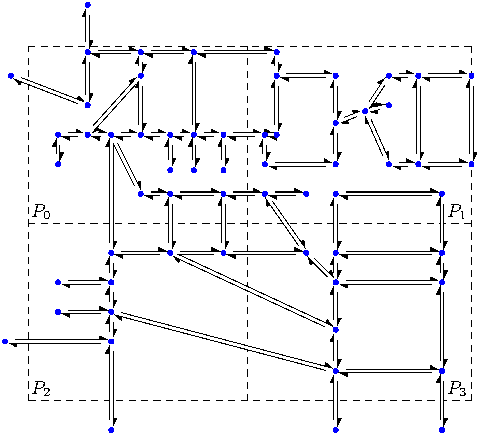
\includegraphics[width=0.75 \linewidth ]{chapterSDCEL/model/ddcel-1}
	\caption{DCEL vertices and half-edges.}
	\label{fig:ddcel:step1}
\end{figure}


\vspace{4pt}
\textit{\textbf{Step 2: Marking the Dangle Half-edges.}}
\\
Dangle half-edges are not part of any face; thus, marking them is essential to exclude them during the polygonization procedure. To find dangles in the input 
lines, we use previously generated information, i.e., information about the vertices and their incident half-edges. 
We compute the degree of each vertex $v \in V$ populated in the previous step. A vertex degree is the number of non-dangle half-edges in its incident half-edges 
list. If the degree of an arbitrary vertex $v$ is less than or equal to 1 ($degree(v) \le 1$), then all of $v$'s incident half-edges and their twins are also 
dangle half-edges. 
Marking any new half-edge as a dangle requires recomputing the degree of the vertices connected to it. 
Thus, marking the dangle half-edges is an iterative process. After the initial run over all vertices and marking the initial dangle half-edges, we reiterate 
over the vertices to check for newly found dangle half-edges. We keep iterating until convergence when no new dangle half-edges are detected.


\vspace{4pt}
\textit{\textbf{Step 3: Setting the Half-edges' Next Pointers, and Marking the Cut Edges.}}
\\
The third step is divided into three smaller steps: (a) setting the next half-edge pointer for each half-edge, (b) marking the cut edges, and (c) updating the 
next half-edges accordingly.
To set the next pointer for each half-edge, we use information from the previous two steps, i.e., the vertices incident half-edges and the current dangle 
half-edges.
For each vertex $v \in V$, we sort its incident half-edges list in clockwise order, excluding the dangle half-edges. 
After sorting the incident half-edges list $v.incidentH$, for every pair of half-edges $v.incidentH[t]$, $v.incidentH[t+1]$ in the sorted list, we assign 
$v.incidentH[t].next$ to $v.incidentH[t+1].twin$. For the last incident half-edge in the sorted list $v.incidentH[v.incidentH.len-1]$, we assign its next 
half-edge to $v.incidentH[0].twin$.


After the initial assignment of the next half-edge pointers, we proceed with the second sub-step, marking the cut edges.
To mark the cut edges, we start our procedure at an arbitrary half-edge $h_{initial}$ and assign our $h_{current}$ half-edge pointer to it. We advance the 
$h_{current}$ pointer at each iteration to the $h_{current}$'s next ($h_{current} = h_{current}.next$), storing all visited half-edges in a list (current 
cycle). We keep advancing the $h_{current}$ pointer till we reach one of three cases.
(1) We return to the initial half-edge $h_{initial}$, which means a cycle is detected and no cut edge is detected.
(2) The half-edge $h_{current}.next$ is not available, which also means no cut edge is detected.
(3) We find $h_{current}.twin$ in the current cycle, which means that $h_{current}$ and its twin are both cut edges. 
Once we reach one of these cases, we mark all visited half-edges as such and proceed with a new arbitrary half-edge to be $h_{initial}$.
This process is terminated when all the partition half-edges are visited.

In the third sub-step, after marking all cut edges, we update the next pointers while excluding the cut edges. 
For each vertex $v \in V$, we sort its incident half-edges list in clockwise order again, now while excluding both the dangle and the cut edge half-edges.
After sorting the incident half-edges list $v.incidentH$, we re-execute the same process of the first sub-step, assigning $v.incidentH[t].next$ to 
$v.incidentH[t+1].twin$. 
Figure~\ref{fig:ddcel:step2} shows the DCEL data structure after removing the dangle and cut edges.


\begin{figure}[tb]
	\centering
	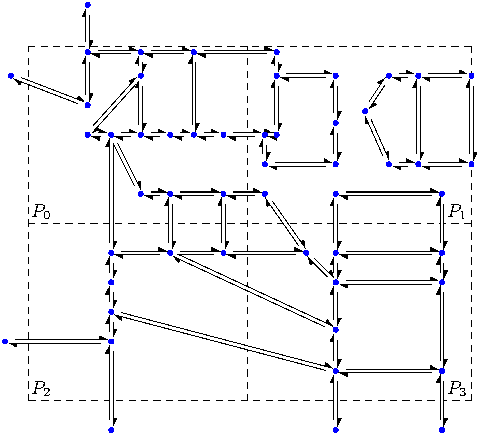
\includegraphics[width=0.75 \linewidth ]{chapterSDCEL/model/ddcel-2}
	\caption{DCEL vertices and half-edges after dangle and cut edge removal.}
	\label{fig:ddcel:step2}
\end{figure}

\vspace{4pt}
\textit{\textbf{Step 4: Generating the Partition Faces.}}
\\
Polygonization on each partition $P_i$ starts with selecting an arbitrary half-edge as our initial half-edge $h_{initial}$.
We initially assign our $h_{current}$ half-edge pointer to $h_{initial}$. We advance the $h_{current}$ pointer at each iteration to the $h_{current}$'s next 
($h_{current} = h_{current}.next$), storing all visited half-edges in a list $cycle$. We keep advancing the $h_{current}$ pointer till we reach one of the 
following cases:
(1) We return to the initial half-edge $h_{initial}$, which means that we have found a face. In this case, we add the found face $f$ to the faces collection 
$F_0$ and assign $h.incidentF = f, \;\; \forall h \in cycle$.
(2) The $h_{current}.next$ is not available, and $h_{current}$ is a half-edge that spans multiple partitions. In this case, the cycle needs more information 
from the neighboring partitions to be completed, and the current partition's data is insufficient to produce this face.
To complete this cycle, we either pass the incomplete cycle into the Rem phase (the current list $cycle$), where it collects all incomplete cycles from all 
partitions and attempts to join them to form a face. Another approach would be passing the plain half-edges in this cycle to the next phase. Both approaches are 
discussed in detail in Section~\ref{sec:rem}.
Once we finish processing this cycle, we mark all visited half-edges as such, clear the cycle, and proceed with a new arbitrary half-edge to be $h_{initial}$.
This process is terminated when all the partition half-edges are visited.
In Figure~\ref{fig:ddcel:faces}, the dotted faces are the faces generated in this phase (Gen Phase).

\begin{figure}[tb]
	\centering
	
\includegraphics[width=0.75 \linewidth ]{chapterSDCEL/model/ddcel-3}
	\caption{DCEL faces.}
	\label{fig:ddcel:faces}
\end{figure}

\subsection{Rem Phase}
\label{sec:rem}

The Rem Phase accepts the remaining half-edges or incomplete cycles as input. 
To be included in the remaining half-edges set, a half-edge cannot be a dangle or a cut edge. Also, the half-edge should not have been bounded to a face yet.
An incomplete cycle is a sequence of half-edges that acts as a candidate face. This incomplete cycle could not be completed since their marginal half-edges span multiple partitions.


The Rem Phase is an iterative phase, where each iteration $j$ generates a subset of faces $F_j$. The unused input data at iteration $j$ is passed to the next iteration $j+1$.
Faces generated from the Gen phase and the Rem phase constitute the whole faces of the subdivision $F$.
In each iteration, the Rem Phase starts with re-partitioning the input data across the worker nodes using a new set of partitions.
This new set of partitions satisfies the convergence criteria; the new number of partitions ($k_j$) at iteration $j$ must be less than the number of partitions ($k_{j-1}$) at iteration $j-1$. This criterion ($k_j < k_{j-1}$) ensures there is an iteration ($m$) at which the remaining line segments are re-partitioned to one partition only, where $m$ is the total number of iterations of the Rem Phase, converging the problem into a sequential one and guaranteeing the termination of the procedure.
After the data re-partitioning, we proceed with generating a subset of the remaining faces. Two approaches are employed for the remaining faces generation, depending on the phase input data.
The first approach assumes the phase input is a set of the \underline{R}emaining \underline{H}alf-edges (RH Approach). 
While the second approach assumes the input is a set of the \underline{I}ncomplete \underline{C}ycles (IC Approach). 

\vspace{4pt}
\textit{\textbf{RH Approach: Iterate over the Remaining Half-edges.}}
\\
At each iteration $j$ and on each new data partition, a subset of the remaining half-edges is received. 
Duplicate half-edges received on one new partition are merged into a single half-edge choosing the half-edge with the available next half-edge.
We follow the same procedure of generating faces in the Gen Phase. Starting from an arbitrary half-edge as our initial half-edge $h_{initial}$, we assign our $h_{current}$ half-edge pointer initially to $h_{initial}$. We advance the $h_{current}$ pointer at each iteration to the $h_{current}$'s next ($h_{current} = h_{current}.next$), storing all visited half-edges in a list $cycle$. We keep advancing the $h_{current}$ pointer till we reach one of the following cases:
(1) We return to the initial half-edge $h_{initial}$, which means that we have found a face. In this case, we add the found face $f$ to the faces collection $F_j$ and assign $h.incidentF = f, \;\; \forall h \in cycle$.
(2) The $h_{current}.next$ is not available, and $h_{current}$ is a half-edge that is not wholly contained in the new partition MBR.
Once we finish processing this cycle, we mark all visited half-edges as such, clear the cycle, and proceed with a new arbitrary half-edge to be $h_{initial}$.
This iteration is terminated when all the remaining half-edges are visited. All half-edges that have not been assigned to any face yet are passed to the next iteration.
The Rem Phase terminates if (1) there are no more remaining half-edges, i.e., all non-dangle non-cut edge half-edges are assigned to a face, or (2) the remaining half-edges have been processed on one partition.

\vspace{4pt}
\textit{\textbf{IC Approach: Iterate over the Incomplete Cycles.}}
\\
At each iteration $j$, and on each new data partition, a subset of the incomplete cycles is received. 
Starting from an arbitrary incomplete cycle $c_{initial}$ with first half-edge $first(c_{initial})$ and last half-edge $last(c_{initial})$, where the first and last half-edges are the incomplete cycle's terminal half-edges, we search for a match $c_{match}$ in the remaining incomplete cycles such that the $last(c_{initial}) = first(c_{match})$. When a match is found, we merge the two cycles such that the $last(c_{initial})$ is now the $last(c_{match})$. We keep merging cycles till we reach one of the following cases:
(1) The $last(c_{match}) = first(c_{initial})$, which means the cycle is now completed. In this case, we add the found face $f$ to the faces collection $F_j$ and remove all incomplete cycles used from the set of the incomplete cycles.
(2) We can not find a match for the current last half-edge, and the last half-edge is not wholly contained within the new partition's MBR. In this case, the incomplete cycle needs more information from the neighboring partitions to be completed, and the current partition's data is insufficient to produce this face.
Once we finish processing this matching process, we mark all visited incomplete cycles as such and proceed with a new arbitrary incomplete cycle to be $c_{initial}$.
This iteration $j$ is terminated when all the incomplete cycles are visited. All incomplete cycles that are not completed yet are passed into the next iteration.
The Rem Phase terminates if (1) there are no more remaining incomplete cycles, i.e., all cycles have been completed, or (2) the incomplete cycles have been processed on one partition.
In Figure \ref{fig:ddcel:faces}, the hatched faces are the faces generated in the first iteration ($j=1$) of the Rem Phase.


\subsection{Data Partitioning}\label{sec:partitioning_ddcel}

The quadtree partitioner is used again to distribute the data amongst the worker nodes across the cluster. In the Gen Phase, the quadtree leaf nodes are used as the initial data partitions.
The output of the Gen Phase, whether the remaining half-edges or the incomplete cycles, is iteratively re-partitioned into new sets of partitions.
Each iteration set of partitions must satisfy the convergence criterion to ensure that the Rem Phase will terminate.
We employ the same quadtree partitioner to generate the new partitions. 
Assume we have a quadtree built on the input line segments of height $L$. 
At the Gen Phase, we use nodes at the leaf level $L$ as our initial data partitions. For each iteration $j$ in the Rem Phase, we level up in the quadtree and choose different level nodes, aside from the leaves, to be our current data partitions.  
We keep leveling up in the quadtree till we reach the root ($l=0$), which means that all data is located on only one partition (the root).
Going up in the quadtree ensures that the number of partitions at iteration $j+1$ is less than that at iteration $j$ since the number of nodes at any arbitrary level $l$ visited at iteration $j$ is more than that at level $l_{chosen}, \ \forall l_{chosen} < l$ visited at iteration $j+1$.


We always start with the leaf nodes level $L$ in the Gen Phase. Choosing which levels to visit next in each iteration $j$ is a system parameter. 
We offer different schemes for the visited quadtree levels: 
\begin{enumerate}
    \item Going directly to the root node at $l=0$ after the leaf nodes, i.e., visiting only levels L in the Gen and 0 in the Rem phases. However, the experimental evaluation shows that collecting the data after the Gen phase on one node is prohibitive, and one worker node will not be able to process the Gen phase's output.
    \item Going \underline{1} \underline{L}evel \underline{U}p (1LU) each iteration, i.e. if we visit level $l$ at iteration $j$, we go to level $l-1$ at iteration $j+1$. This means the Rem Phase visits all the quadtree levels resulting in $L$ iterations.
    \item Going \underline{2} \underline{L}evels \underline{U}p (2LU) each iteration resulting in half the number of iterations $\frac{L}{2}$ compared to 1LU.
    \item Skipping to the \underline{M}iddle of the tree at level $\frac{L}{2}$, then continue going 1 level up for the remaining levels (M1LU), which will also result in $\frac{L}{2}$ iterations.
    \item Skipping to the \underline{M}iddle of the tree every time, dividing the current level by two each iteration (MU); this will result in $\log_2(L)$ iterations.
\end{enumerate}
The goal is to find a re-partitioning scheme with a minimal number of iterations, thus reducing the workload of the Rem Phase while ensuring that the worker nodes can process the chunk of the data it receives at each iteration $j$.
The extreme case of having only one iteration at the Rem Phase will not work since the data is too big to fit one partition and be processed by only one worker node. On the other hand, the more unnecessary iterations we have, the more overhead on the system resulting in higher query latency.


\subsection{Overlaying Polygons with Dangle and Cut Edges} \label{sec:over_dang}

\begin{figure}[tb]
	\centering
	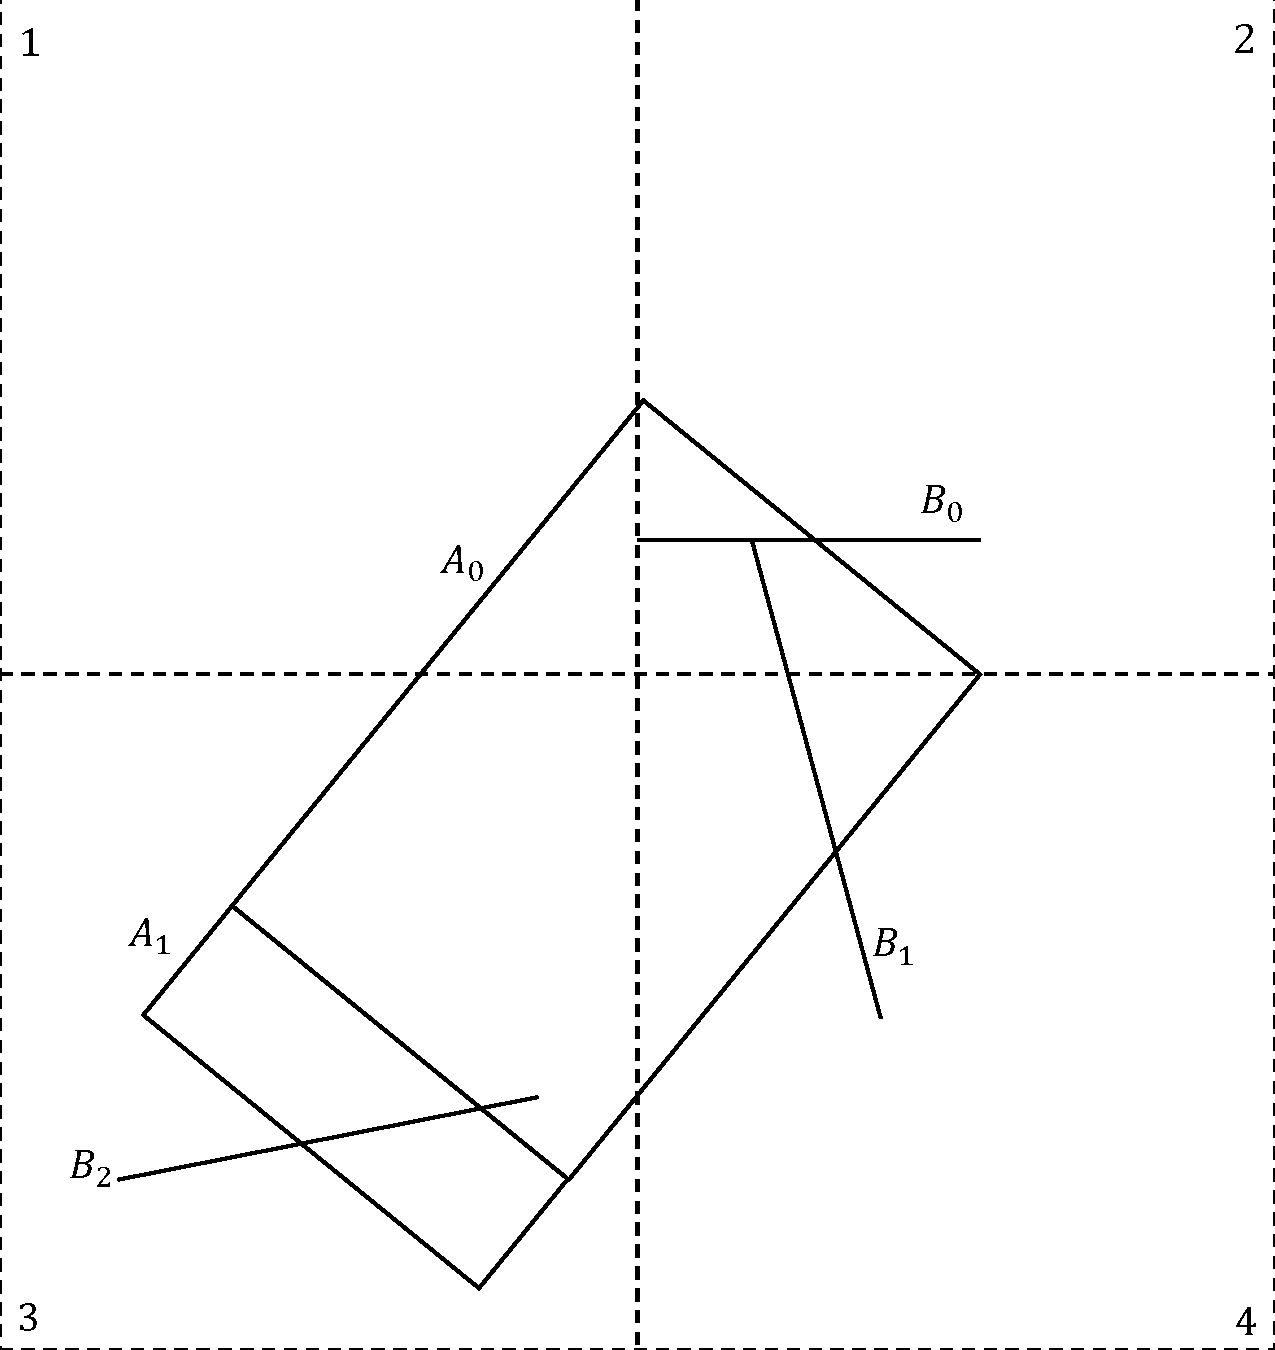
\includegraphics[width=0.75 \linewidth ]{chapterSDCEL/model/DangleOverlay1.pdf}
	\caption{Spatial partitioning of input layers A and B}
	\label{fig:dangleoverlay:input}
\end{figure}

\begin{figure}[tb]
	\centering
	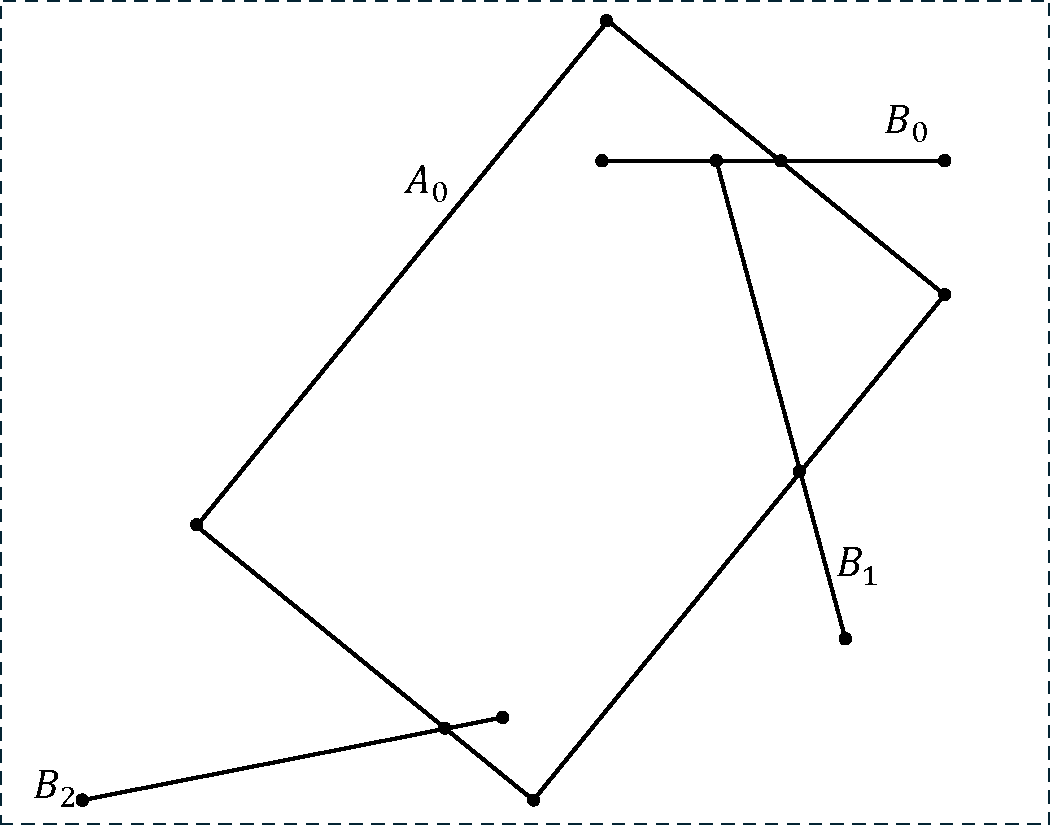
\includegraphics[width=0.75 \linewidth ]{chapterSDCEL/model/DangleOverlay2.pdf}
	\caption{Re-Partitioning of polygon $A_0$ with edges it intersects with}
	\label{fig:dangleoverlay:inter}
\end{figure}

\begin{figure}[tb]
	\centering
	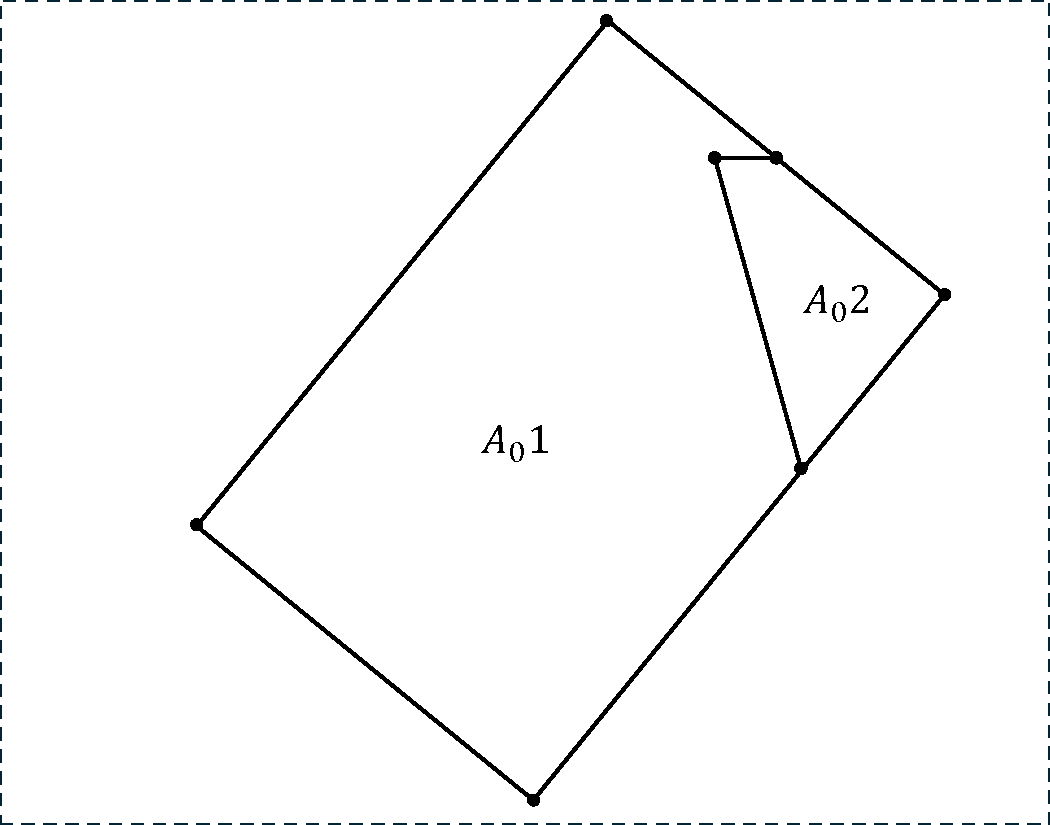
\includegraphics[width=0.75 \linewidth ]{chapterSDCEL/model/DangleOverlay3.pdf}
	\caption{The result of polygonization of $A_0$ with $B_0, B_1, B_2$}
	\label{fig:dangleoverlay:result}
\end{figure}

The polygonization procedure produces two outputs: first, a set of closed polygons formed by the input planar line segments, and second, any edges that are not 
a part of any polygon, i.e., dangle or cut edges. 
Overlaying the polygons generated with any polygon layer follows the approaches discussed in sections \ref{sec:methods} and \ref{sec:alternative_methods}.
However, we need to modify the algorithms provided in these previous sections to overlay an input polygon layer $A$ with the dangle and cut edges, i.e. layer 
$B$. In particular, we modify the reduce phase.
Figure \ref{fig:dangleoverlay:input} illustrates the spatial partitioning of the two input layers, $A$ and $B$. Layer $A$ contains two input polygons, $A_0$ and 
$A_1$, while Layer $B$ consists of three dangle edges, $B_0$, $B_1$, and $B_2$.

Each edge from layer $B$ is labeled a unique label and is fed as an input to the overlay module.
The local overlay is performed by finding intersections between the input polygon layer $A$ and layer $B$ on each data partition.
If a polygon with $id = i$ from polygon layer $A$ intersects with edges with ids $id = a, id = b, id = c$ from layer $B$ at some data partition, we generate a 
label to match these intersections $A_{i} B_{a} B_{b} B_{c}$. 
At the reduce phase, we re-partition the data by the first label, meaning we collect all edges that intersect with the first label.
If two data partitions produced the labels $A_{i} B_{a} B_{b} B_{c}$ and $A_{i} B_{x} B_{y}$, we repartition the data such that $A_{i}$ is on one partition with 
all edges it is intersecting, i.e., $B_{a}, B_{b}, B_{c}, B_{x}, B_{y}$.
In Figure \ref{fig:dangleoverlay:inter}, Polygon $A_0$ is re-partitioned along with the edges it intersects, specifically $B_0$, $B_1$, and $B_2$.

After re-partitioning the data, we have all edges from both layers intersecting each other on the same partition. The next step is to find the polygons 
generated by these intersections. Since there is no guarantee that only one polygon is generated, we substitute the polygon concatenation proposed in 
Section~\ref{sec:reduce} by performing \textit{polygonization} on each partition. The polygonization procedure ensures it generates all new possible polygons. 
The polygonization procedure follows the algorithm mentioned in Section~\ref{sec:gen}. It starts with generating the new vertices and half-edges, then marking 
the current dangles and cut edges, then setting the next pointers and finally generating the partition polygons.
Figure \ref{fig:dangleoverlay:result} shows the result of polygonizing the edges from Polygon $A_0$ and $B_0$, $B_1$, and $B_2$, resulting in two polygons, 
$A_01$ and $A_02$.

Polygons from all partitions generate the overlay between the polygon layer $A$ and layer $B$.

\section{Experimental Evaluation} \label{sec:experiments}
For our experimental evaluation, we used a 12-node Linux cluster (kernel 3.10) and Apache Spark 2.4. Each node has 9 cores (each core is an Intel Xeon CPU at 1.70GHz) and 2G memory.

The scalable approach was implemented over the Apache Spark framework.  From a Map-Reduce point of view the stages described in Section \ref{sec:methods} were implemented using several transformations and actions supported by Apache Spark.  For example, the partitioning and load balancing described in Section \ref{sec:pstrategies} was implemented using a quadtree, where its leaves were used to map and balance the number of edges that have to be sent to the worker nodes.  Mostly, map operations were used to process and locate the edges in the corresponding leaf to exploit proximity among them while at the same time dividing the amount of work among worker nodes.

Similarly, the edges at each partition were processed using chains of transformations at local level (see Section \ref{sec:methods}) followed by reducer actions to post-process incomplete faces which could span over multiples partitions and have to be combined or re-distributed to obtain the final answer.  In addition, the reduce actions were further optimized as described in Section \ref{sec:alternative_methods}.

\subsection{Evaluation datasets}
The details of the real datasets of polygons that we use are summarized in Table \ref{tab:sdcel_datasets}. The first dataset (MainUS) contains the complete Census Tracts for all the states on the US mainland for the years 2000 (layer A) and 2010 (layer B). It was collected from the official website of the United States Census Bureau \cite{census_tract}. The data was clipped to select just the states inside the continent. Something to note with this dataset is that the two layers present a spatial gap (which was due to improvements in the precision introduced for 2010). As a result, there are considerably more intersections between the two layers, thus creating many new faces for the DCEL.

\begin{table}
    \centering
    \caption{Evaluation Datasets}
    \label{tab:sdcel_datasets}
    \begin{tabular}{c c c c}
        \toprule
        Dataset & Layer & Number        & Number    \\
                &       & of polygons   & of edges  \\
        \midrule
        MainUS& Polygons for 2000 & 64983 & 35417146        \\
              & Polygons for 2010 & 72521 & 36764043        \\
        GADM  & Polygons for Level 2 & 160241 & 64598411    \\
              & Polygons for Level 3 & 223490 & 68779746    \\
        CCT   & Polygons for 2000 & 7028 & 2711639          \\
              & Polygons for 2010 & 8047 & 2917450          \\
        \bottomrule
    \end{tabular}
\end{table}

The second dataset, GADM - taken from Global Administration Areas \cite{gadm_data}, collects the geographical boundaries of the countries and their administrative divisions around the globe. For our experiments, one layer selects the States (administrative level 2), and the other has Counties (administrative level 3). Since GADM may contain multi-polygons, we split them into their individual polygons.

Since these two datasets are too large, a third, smaller dataset was created for comparisons with the sequential algorithm. This dataset is the California Census Tracts (CCT), a subset from MainUS for the state of California; layer A corresponds to the CA census tracts from the year 2000, while layer B corresponds to 2010. Below, we also use other states to create datasets with different numbers of faces.  To test the scalable approach, a sequential algorithm for DCEL creation was implemented based on the pseudo-code outlined in \cite{berg_computational_2008}.

\subsection{Overlay face optimizations}\label{sec:overlay_optimization}
We first examine the optimizations in Section \ref{sec:optimizing}. To consider different distributions of faces, for these experiments, we used 8 states from the MainUS dataset with different numbers of tracts (faces). In particular, we used, in decreasing order of number of tracts, CA, TX, NC, TN, GA, VA, PA, and FL. For each state, we computed the distributed overlay between two layers (2000 and 2010). For each computation, we compared the baseline; master at the root node, with intermediate reducers at different levels: $i$ varied from 4 to 10. 

Figure \ref{fig:overlay_tester} shows the results for the distributed overlay computation stage; after the local DCELs were computed at each cell. 
Note that for each state experiment, we tested different numbers of cells for the quadtree and reported the configuration with the best performance. To determine this, we sampled 1\% of the edges for each state and evaluated the best number of cells ranging from 200 to 2000. In most cases, the best number of cells was around 3000.
As expected, there is a trade-off between parallelism and how much work is left to the final reduce job. For different states, the optimal $i$ varied between levels 4 and 6. The figure also shows the optimization that re-partitions the faces by label id. This approach has actually the best performance. This is because few faces with the same label can be combined independently. This results in smaller jobs better distributed among the cluster nodes, and no reduce phase is needed. As a result, we use the label re-partition approach for the rest of the experiments to implement the overlay computation stage.

\begin{figure}
    \centering
    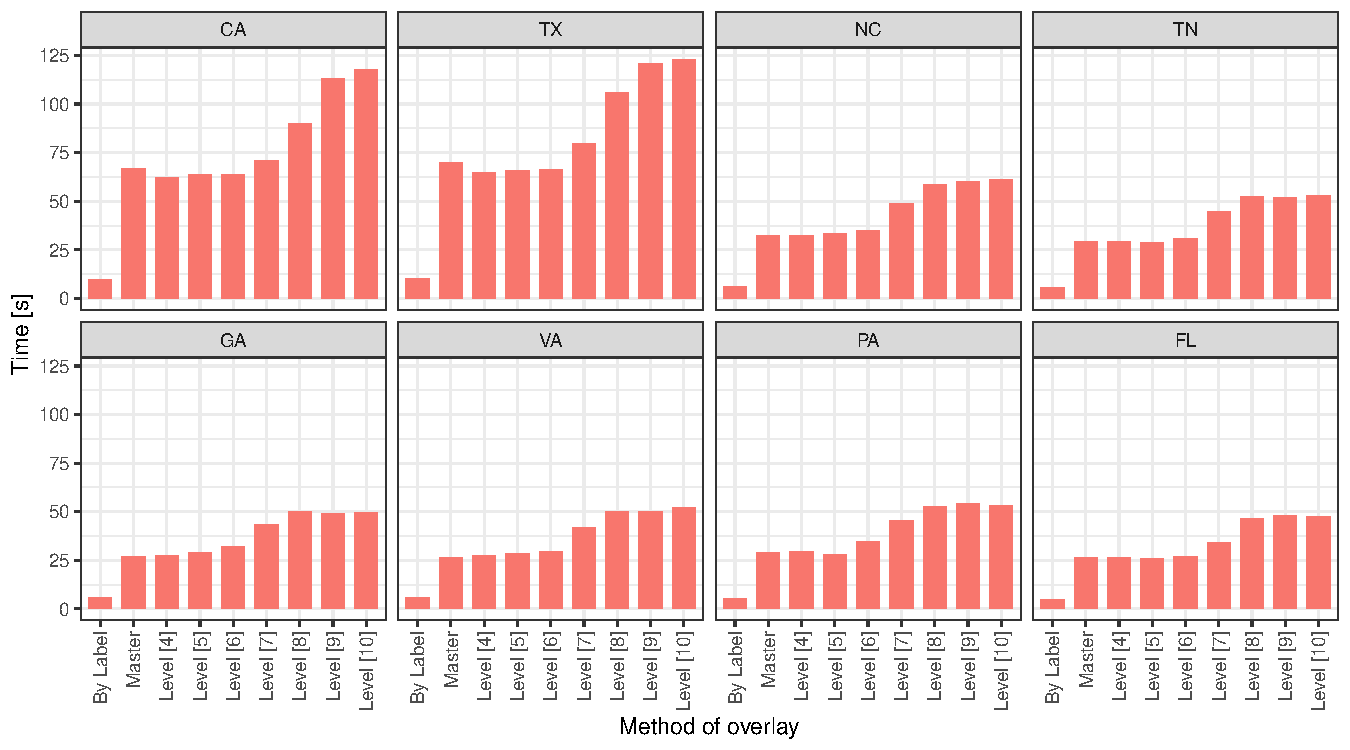
\includegraphics[width=\linewidth]{chapterSDCEL/OverlayTester/Overlay_Tester}
    \caption{Overlay methods evaluation.}\label{fig:overlay_tester}
\end{figure}

Finally we note that the overlay face optimizations involve shuffling of the incomplete faces. Table \ref{tab:percentages} shows the percentage of incomplete faces for three states, assuming 3000 cells. As it can be seen, the incomplete faces is small (in average 12.89\%) and moreover, for the \textit{By-Label} approach, this shuffling is parallelized.

\begin{table}
    \centering
    \caption{Percentages of edges in incomplete faces for three states} \label{tab:percentages}
    \begin{tabular}{cccc}
        \toprule
                & Number of & Edges in         &            \\
        Dataset & edges     & incomplete faces & Percentage \\
        \midrule
        CA &  47834 &  6339 & 13.25\% \\
        TX &  41227 &  4436 & 10.75\%\\
        FL &  24152 &  3547 & 14.68\%\\
        \bottomrule
    \end{tabular}
\end{table}

\subsection{Unbalanced layers optimization}
For these experiments, we compared the traditional sweep approach with the `filtered-sweep' approach that considers only the areas where the smaller layer has edges (Section \ref{sec:unbalance}).  To create the smaller cell layer, we picked a reference point in the state of Pennsylvania, from the MainUS dataset, and added 2000 census tracts until the number of edges reached 3K. We then varied the size of the larger cell layer in a controlled way: using the same reference point but using data from the 2010 census, and we started adding tracts to create a layer that had around 2x, 3x, ..., 7x the number of edges of the smaller dataset.

Since this optimization occurs per cell, we used a single node to perform the overlay computation within that cell. Figure \ref{fig:unbalance_tests}(a) shows the behavior of the two methods (filtered-sweep vs. traditional sweep) under the above-described data for the overlay computation stage.  Clearly, as the data from one layer grows much larger than the other layer, the filtered-sweep approach overcomes the traditional one.

\begin{figure}
    \centering
    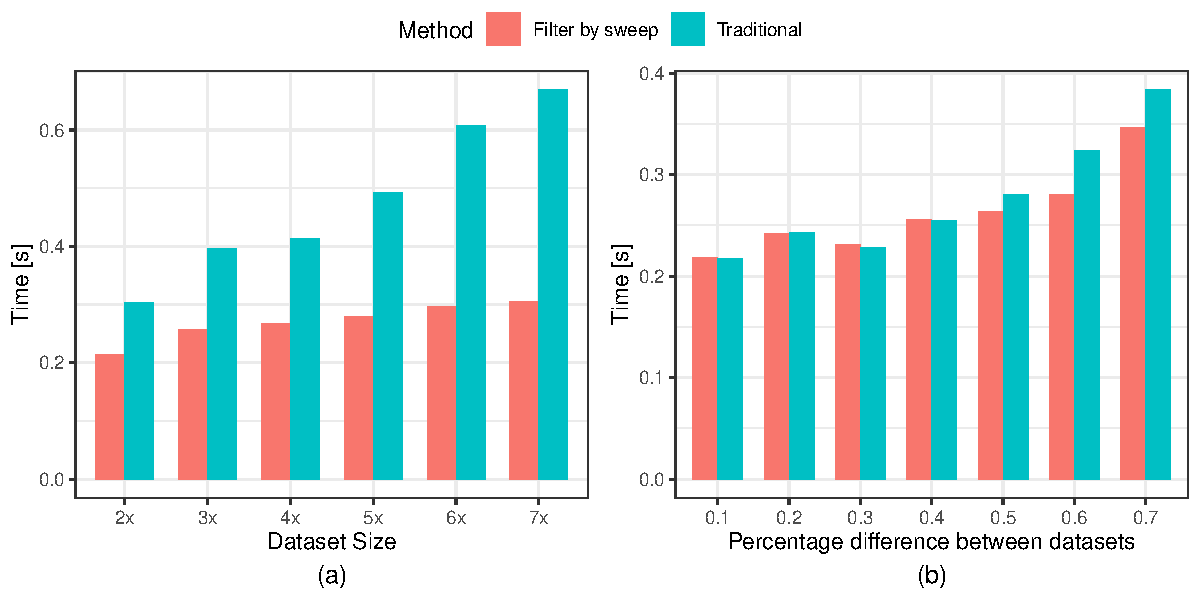
\includegraphics[width=\linewidth]{chapterSDCEL/UnbalanceTester/Unbalance_Tester}
    \caption{Evaluation of the unbalanced layers optimization.}\label{fig:unbalance_tests}
\end{figure}

We also performed an experiment where the difference in size between the two layers varies between 10\% and 70\%. For this experiment, we first identified cells from the GADM dataset where the smaller layer had around 3K edges. Among these cells, we then identified those where the larger layer had 10\%, 20\%, ... up to 70\% more edges. In each category, we picked 10 representative cells and computed the overlay for the cells in that category.

Figure \ref{fig:unbalance_tests}(b) shows the results; in each category, we show the average time to compute the overlay among the 10 cells in that category.  The filtered-sweep approach shows better performance as the percentage difference between layers increases. Based on these results, one could apply the optimization on those cells where the layer difference is significant (more than 50\%).  We anticipate that this optimization will be particularly beneficial for datasets where the two input layers contain many cells with significantly different edge counts.

\subsection{Varying the number of cells}
The quadtree configuration allows for performance tuning by setting the \textit{maximum capacity} of a cell. The quadtree continues splitting until this capacity is reached. There is an inverse relationship between the capacity and the number of leaf cells: a lower capacity results in more cells, while a higher capacity leads to fewer leaf cells. In skewed datasets, the quadtree may become unbalanced, with some branches splitting more frequently. As a result, the final number of partitions is not necessarily a multiple of four. In the figures, we round the number of leaf cells to the nearest thousand.

The number of cells affects the performance of our scalable overlay implementation, termed as SDCEL, since it relates to the average cell capacity given by the number of edges it could contain. As it was said before, a fewer number of cells implies larger cell capacity and thus more edges to process within each cell.  Complementary, creating more cells increases the number of jobs to be executed.

Figure \ref{fig:ca}(a) shows the SDCEL performance using the two layers of the CCT dataset while varying the number of cells from 100 to 15K (by multiple of 1000). Each bar corresponds to the time taken to create the DCEL for each layer and then combine them to create the distributed overlay. Clearly, there is a trade-off: as the number of cells increases, the SDCEL performance improves until a point where the larger number of cells adds an overhead. Figure \ref{fig:ca}(b) focuses on that area; the best SDCEL performance was around 7K cells.

In addition, Figure \ref{fig:ca}(a) shows the performance of the sequential solution (CGAL library) for computing the overlay of the two layers in the CCT dataset using one of the cluster nodes. Clearly, the scalable approach is much more efficient as it takes advantage of parallelism. Note that the CGAL library would crash when processing the larger datasets (MainUS and GADM).

\begin{figure}
    \centering
    \begin{tabular}{cc}
        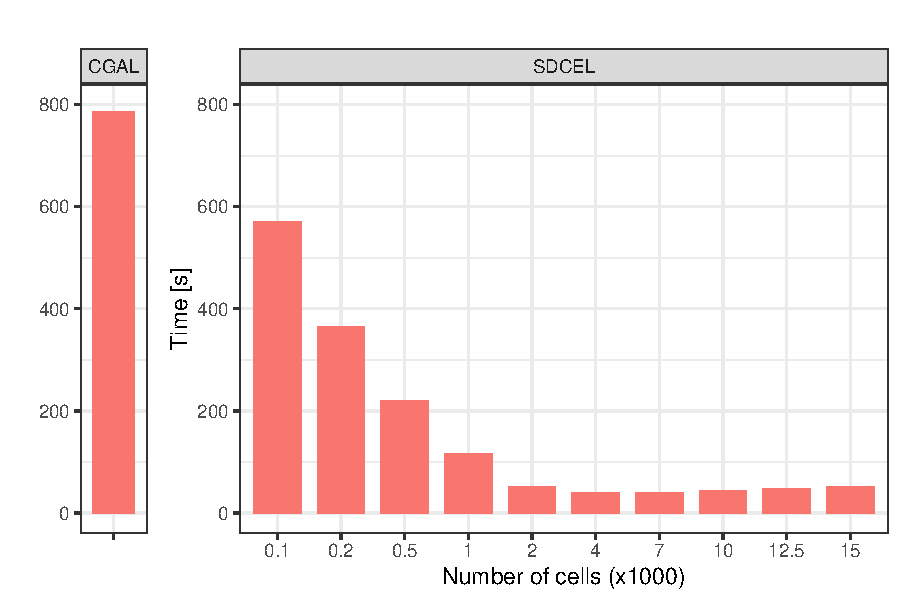
\includegraphics[width=0.50\linewidth]{chapterSDCEL/CA/CA} & 
        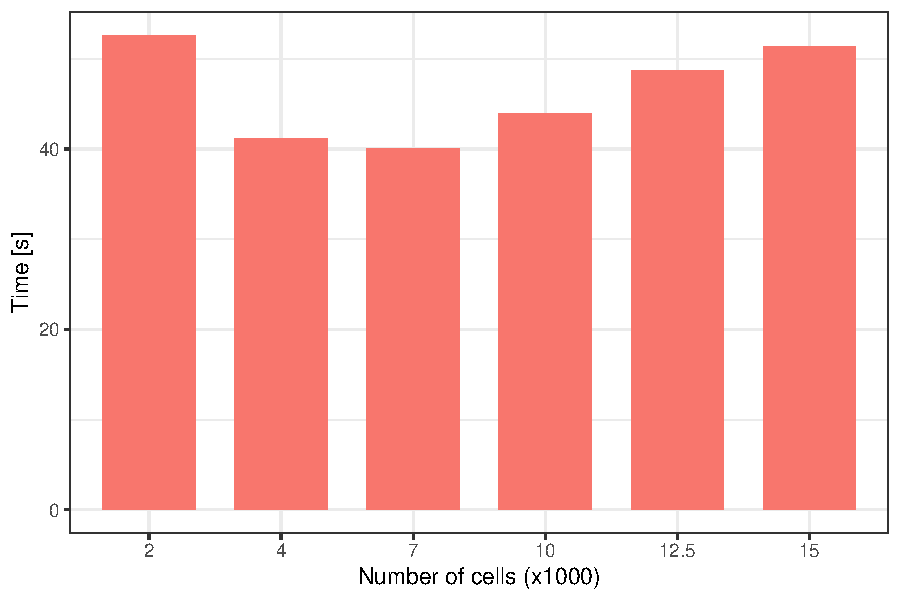
\includegraphics[width=0.45\linewidth]{chapterSDCEL/CA/CA_sample} \\
        (a) & (b)
    \end{tabular}
    \caption{SDCEL performance while varying the number of cells in the CCT dataset.} \label{fig:ca}
\end{figure}

\begin{figure}
    \centering
    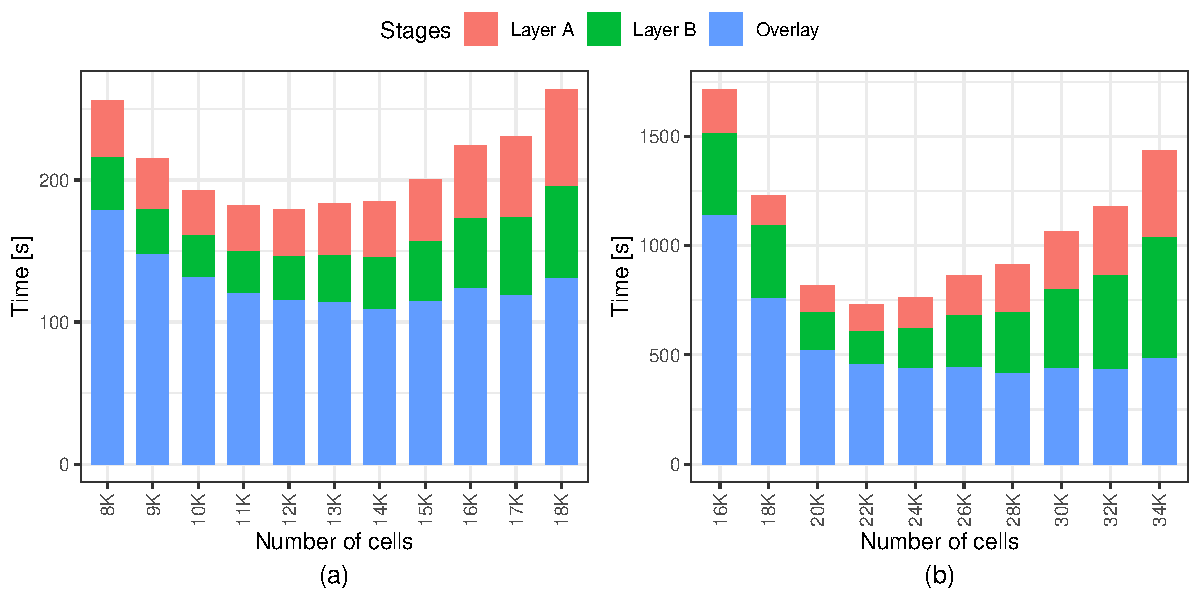
\includegraphics[width=\textwidth]{chapterSDCEL/Performance/Performance} 
    \caption{Performance with (a) MainUS and (b) GADM datasets.} \label{fig:mainus}
\end{figure}

Figure \ref{fig:mainus} shows the results when using the larger MainUS and GADM datasets, while again varying the number of cells parameter from 8K to 18K and from 16K to 34K, respectively. In this figure, we also show the time taken by each stage of the overlay computation.  This is, the time to create the DCEL for layer A, for layer B, and for their combination to create their distributed overlay. We can see a similar trade-off in each of the stages. The best performance is given when setting the number of cells parameter to 12K for the MainUS and 22K for the GADM dataset. Note that in the MainUS dataset, the two layers have a similar number of edges; as can be seen, their DCEL computations are similar.

Interestingly, the overlay computation is expensive since as mentioned earlier there are many intersections between the two layers. An interesting observation from the GADM plots is that layer B takes more time than layer A; this is because there are more edges in the counties than in the states. Moreover, county polygons are included in the (larger) state polygons. When the size of cells is small (i.e., a larger number of cells like in the case of 34K cells), these cells mainly contain counties from layer B. As a result, there are not many intersections between the layers in each cell, and the overlay computation is thus faster. On the other hand, with large cell sizes (smaller number of cells), the area covered by the cell is larger, containing more edges from states and thus increasing the number of intersections, resulting in higher overlay computation.

Additionally, Table \ref{tab:cell_stats} provides statistics on the cells. It shows that in larger datasets, an average cell size of approximately 3000 edges produces the best results. This cell size ensures a relatively small amount of data to transmit, which minimizes the impact on data shuffling and processing.  Table \ref{tab:orphans} presents the number of cells, original holes, and the orphan cells and holes generated after partitioning.

\begin{table}
    \centering
    \caption{Cell size statistics.}
    \label{tab:cell_stats}
    \begin{tabular}{ccccccc}
        \toprule
        Dataset & Min & 1st Qu. & Median & Mean & 3rd Qu. & Max   \\
        \midrule
        GADM    & 0   & 0       & 2768   & 3141 & 5052    & 16978 \\
        MainUS  & 0   & 1538    & 2582   & 2853 & 3970    & 10944 \\
        CCT     & 0   & 122     & 324    & 390  & 546     & 1230  \\
        \bottomrule
    \end{tabular}
\end{table}

\begin{table}
    \centering
    \caption{Orphan cells and orphan holes description}
    \label{tab:orphans}
    \begin{tabular}{c c c c}
        \toprule
                & Number   & Number   & Number of orphans   \\
        Dataset & of cells & of holes & (cell/holes) \\
        \midrule
        GADM  & 21970      & 1999     & 4310 \\
        MainUS& 12343      & 850      & 1069 \\
        CCT   & 7124       & 40       & 215  \\
        \bottomrule
    \end{tabular}
\end{table}

\subsection{Speed-up and Scale-up experiments} \label{sec:speed_scale}
The speed-up behavior of SDCEL appears in Figure \ref{fig:mainus_speed_scale}(a) (for the MainUS dataset) and in Figure \ref{fig:gadm_speed_scale}(a) (for the GADM dataset); in both cases, we show the performance for each stage. For these experiments, we varied the number of nodes to 3, 6, and 12 while keeping the input layers the same. Clearly, as the number of nodes increases, the performance improves. SDCEL shows good speed-up characteristics: as the number of nodes doubles from 3 to 6 and then from 6 to 12, the performance improves by almost half.

\begin{figure}
    \centering
    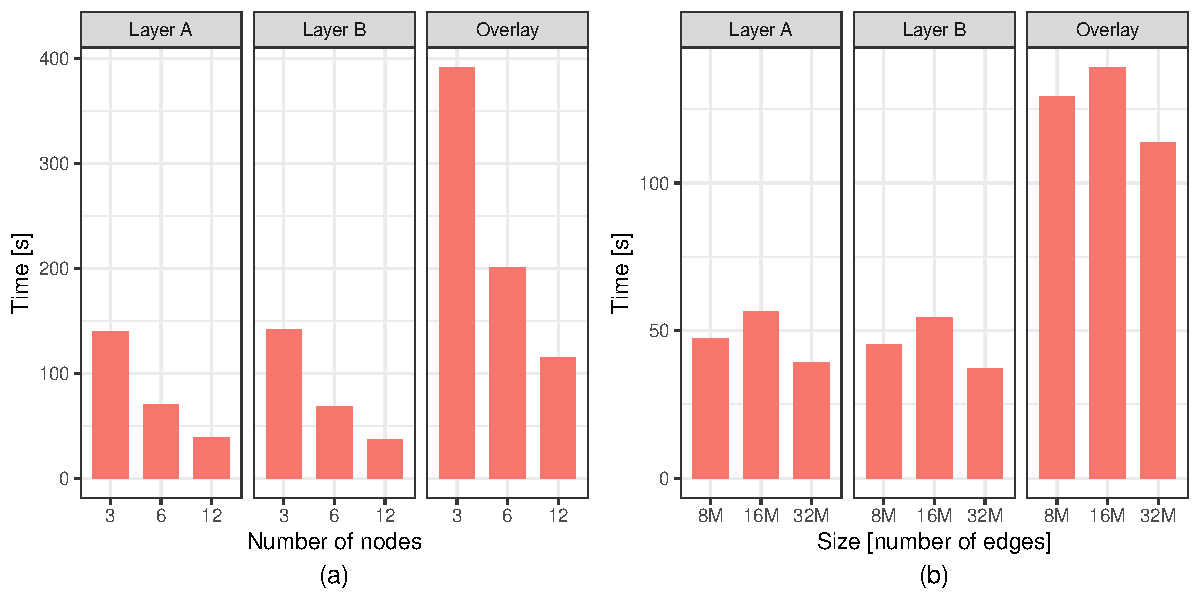
\includegraphics[width=\textwidth]{chapterSDCEL/MainUS_SS/MainUS_SS} 
    \caption{Speed-up and Scale-up experiments for the MainUS dataset.} 
\label{fig:mainus_speed_scale}
\end{figure}

\begin{figure}
    \centering
    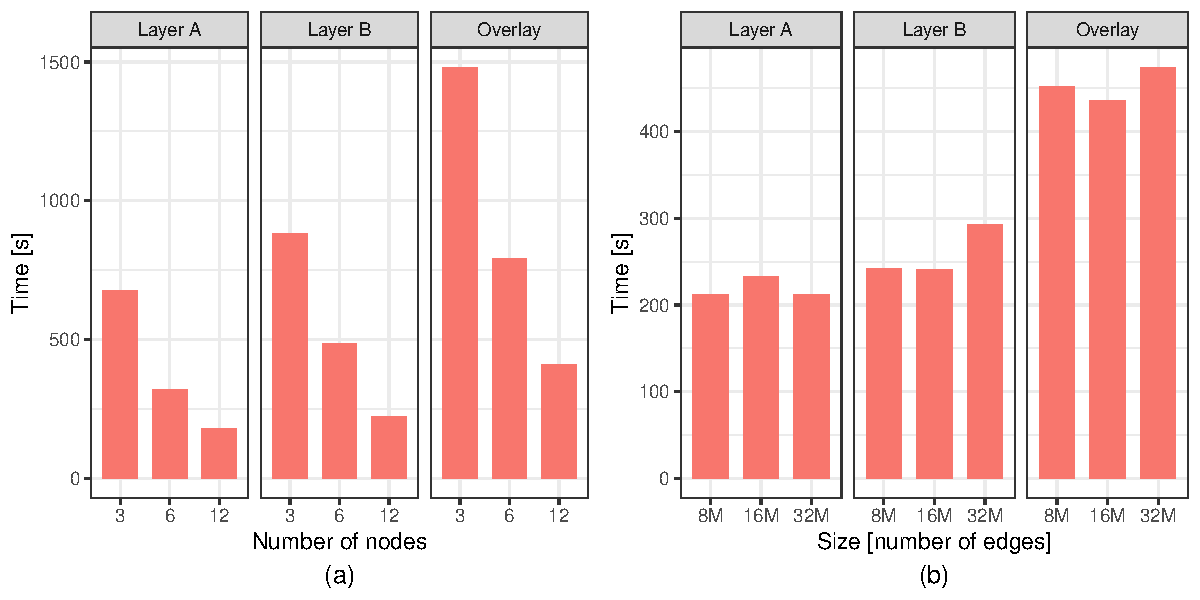
\includegraphics[width=\textwidth]{chapterSDCEL/GADM_SS/GADM_SS}
    \caption{Speed-up and Scale-up experiments for the GADM dataset.} \label{fig:gadm_speed_scale}
\end{figure}

To examine the scale-up behavior, we created smaller datasets out of the MainUS and similarly out of the GADM so that we could control the number of edges. To create such a dataset, we picked a centroid and started increasing the area covered by this dataset until the number of edges was closed to a specific number. For example, from the MainUS, we created datasets of sizes 8M, 16M, and 32M edges for each layer. We then used two layers of the same size as input to a different number of nodes while keeping the input-to-node ratio fixed. That is, the layers of size 8M were processed using 3 nodes, the layers of size 16M using 6 nodes, and the 32M using 12 nodes. We used the same process for the scale-up experiments with the GADM dataset. The results appear in Figure \ref{fig:mainus_speed_scale}(b) and Figure \ref{fig:gadm_speed_scale}(b).  Overall, SDCEL shows good scale-up performance; it remains almost constant as the work per node is similar (there are slight variations because we could not control perfectly the number of edges and their intersection).

%% Extension
%\subsection{Kd-tree versus quadtree performance} \label{sec:comparison}
%In order to compare the quadtree and the kd-tree partition strategies we analyze their performance during the construction of the spatial data structure which defines the cells that the partition will use based on the sample, the cost of partitioning; populating the cells with the full datasets, and the overall time to complete the phases of the overlay operation using each partitioning approach.  We use the datasets of MainUS and GADM described in Table \ref{tab:datasets}.

% \begin{figure}
%     \centering
%     \begin{tabular}{cc}
%         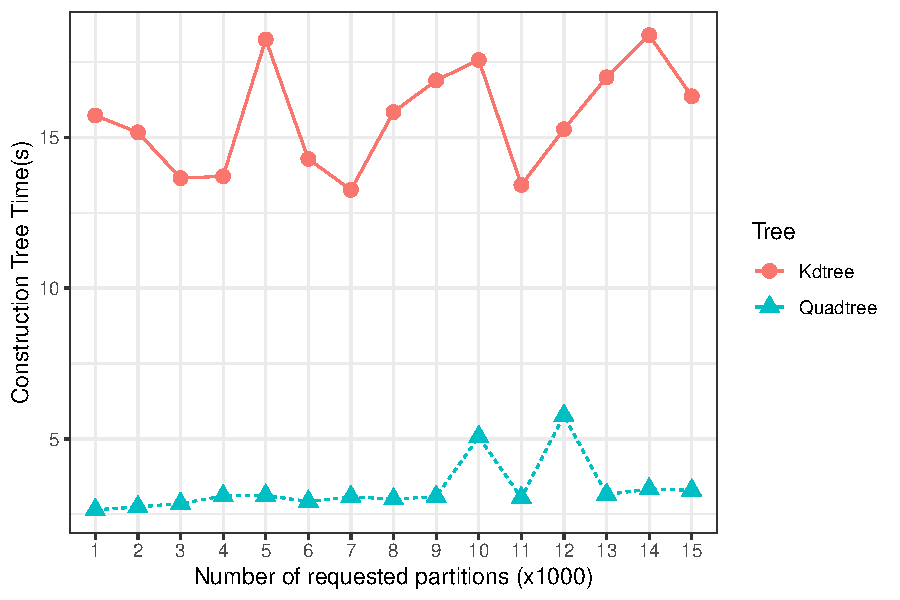
\includegraphics[width=0.49\linewidth]{chapterSDCEL/K_Creation_US.pdf} & 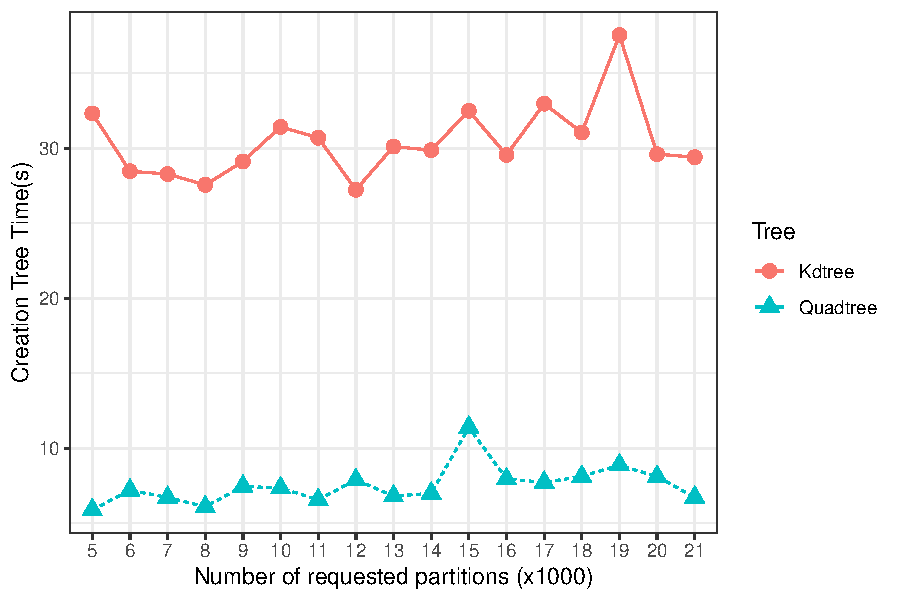
\includegraphics[width=0.49\linewidth]{chapterSDCEL/K_Creation_GADM.pdf} \\
%         (a) & (b)
%     \end{tabular}
%     \caption{Construction time for the spatial data structure in the (a) MainUS and (b) GADM datasets.} \label{fig:k_creation_us}
% \end{figure}

% \begin{figure}
%     \centering
%     \begin{tabular}{cc}
%         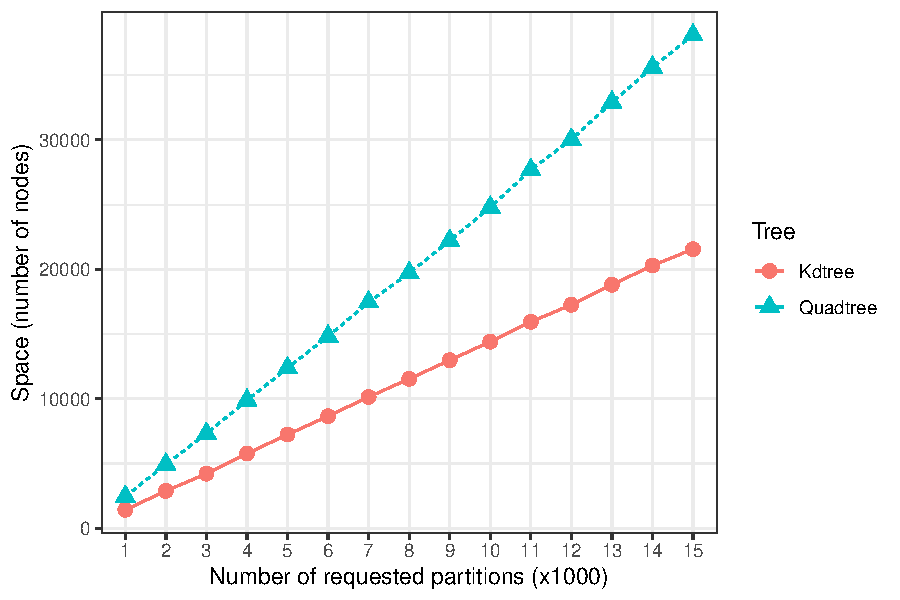
\includegraphics[width=0.49\linewidth]{chapterSDCEL/K_Space_US.pdf} & 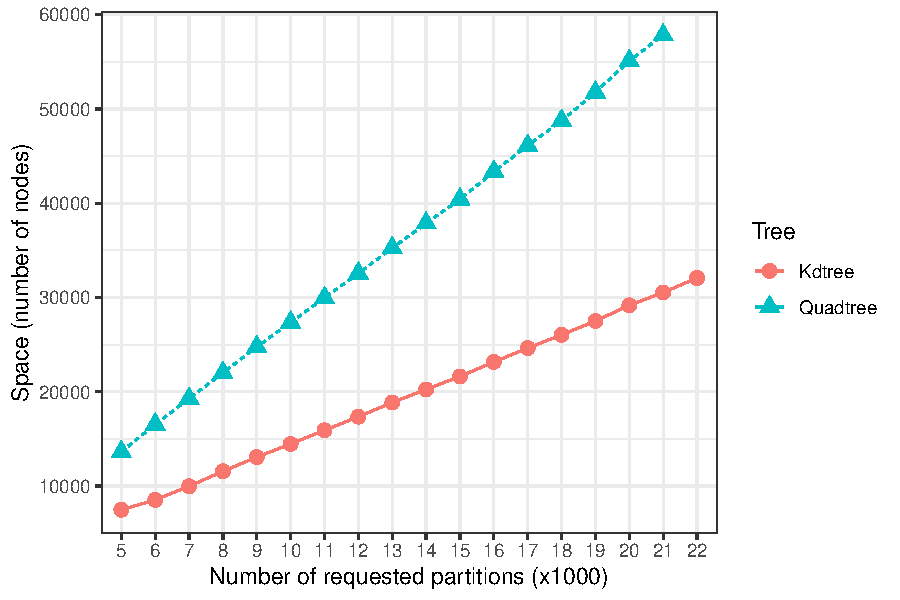
\includegraphics[width=0.49\linewidth]{chapterSDCEL/K_Space_GADM.pdf} \\
%         (a) & (b)
%     \end{tabular}
%     \caption{Number of cells created by each spatial data structure in the (a) MainUS and (b) GADM datasets.} \label{fig:k_space_us}
% \end{figure}

% Figure \ref{fig:k_creation_us} depicts the construction time during the sampling of the input layers and the generation of the partitioning cells after requesting a different number of divisions. We can see that the kd-tree takes more time, particularly because of the sorting done at each split, so as to organize the data and localize the middle point. In average, Quadtree takes 23.13\% the time it takes for Kdtree to be created (21.55\% in MainUS and 24.72\% in GADM). However, the Kdtree creation is just 5.86\% of the overall time during the total DCEL construction (6.88\% in MainUS and 4.87\% in GADM).

% \begin{figure}
%     \centering
%     \begin{tabular}{cc}
%         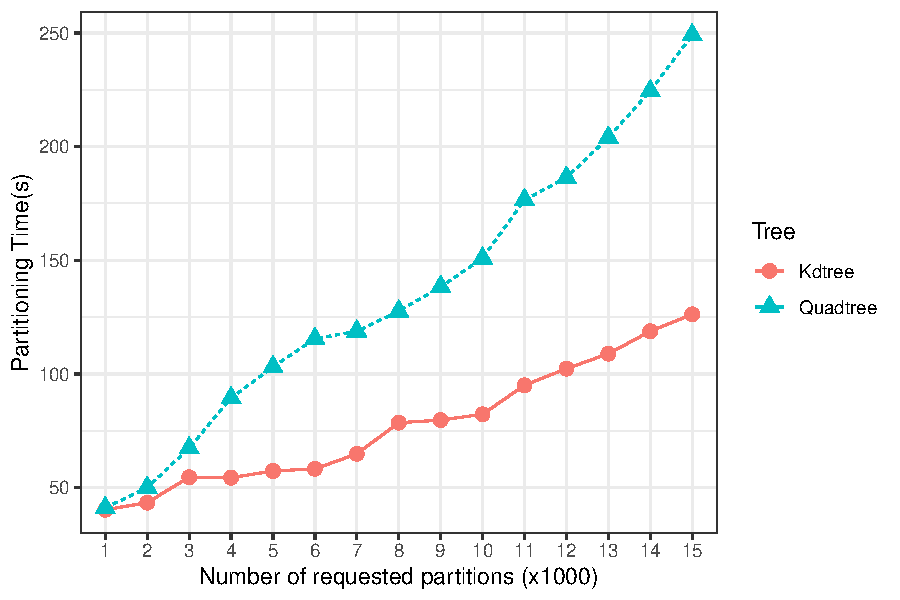
\includegraphics[width=0.49\linewidth]{chapterSDCEL/K_Partitioning_US.pdf} &
%         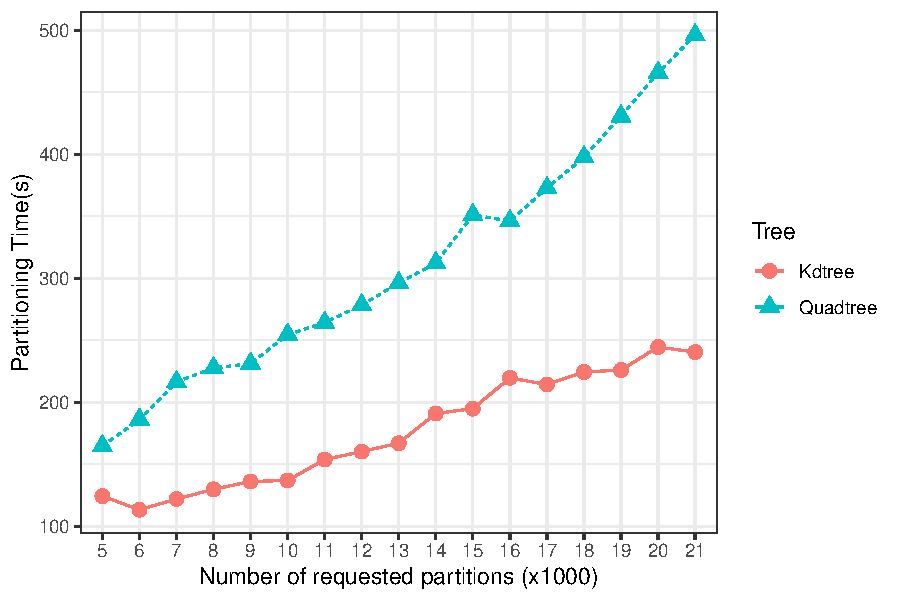
\includegraphics[width=0.49\linewidth]{chapterSDCEL/K_Partitioning_GADM.pdf} \\
%         (a) & (b)
%     \end{tabular}
%     \caption{Data partitioning time using a spatial data structure (a) in the MainUS dataset and (b) in the GADM dataset.} \label{fig:k_partitioning_us}
% \end{figure}

%An important characteristic of the behavior of each partitioning scheme is the number of cells (partitions) each sample data structure creates. Figure \ref{fig:k_space_us} depicts the number of cells created by each spatial data structure. As the quadtree follows a space-oriented technique, it creates more nodes (4 at each split) and thus generates more leaves (cells); more of them are prone to be empty compared to the kd-tree.

%Figure \ref{fig:k_partitioning_us} shows the cost to partition the full content of both layers. Given a sample tree data structure, each edge is assigned to a cell (partition) depending on which leaf the edge is located; edges are assigned (copied) to all leaves they intersect. Then, a shuffle operation is performed to move the data to the corresponding node that will handle this cell (partition). This figure shows that the quadtree partitioning takes more time. This depends largely on the number of leaves created by the sample tree and the number of edges that overlap partitions (which is expected to be larger for the quadtree since it uses more and thus smaller cells).

% \begin{figure}
%     \centering
%     \begin{tabular}{cc}
%         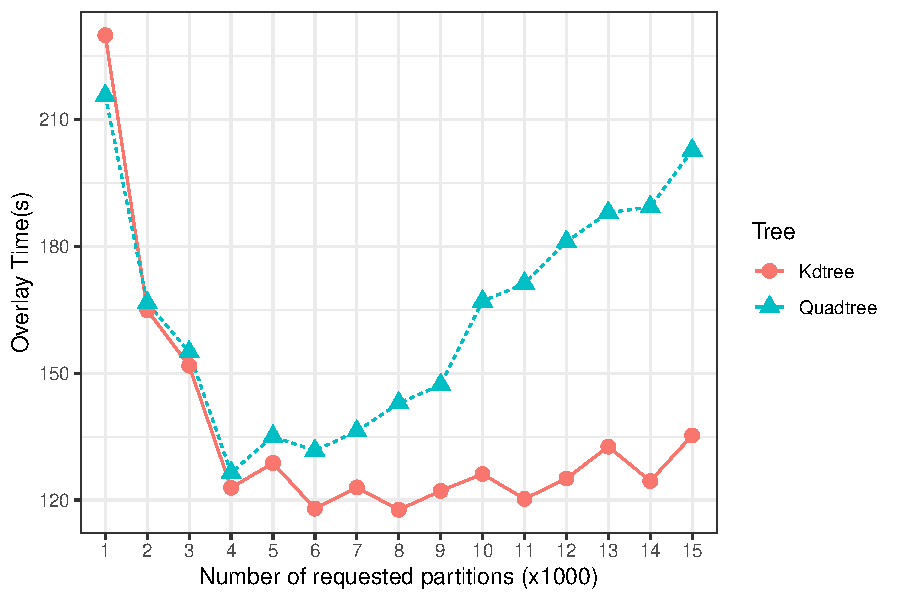
\includegraphics[width=0.49\linewidth]{chapterSDCEL/K_Overlay_US.pdf} &
%         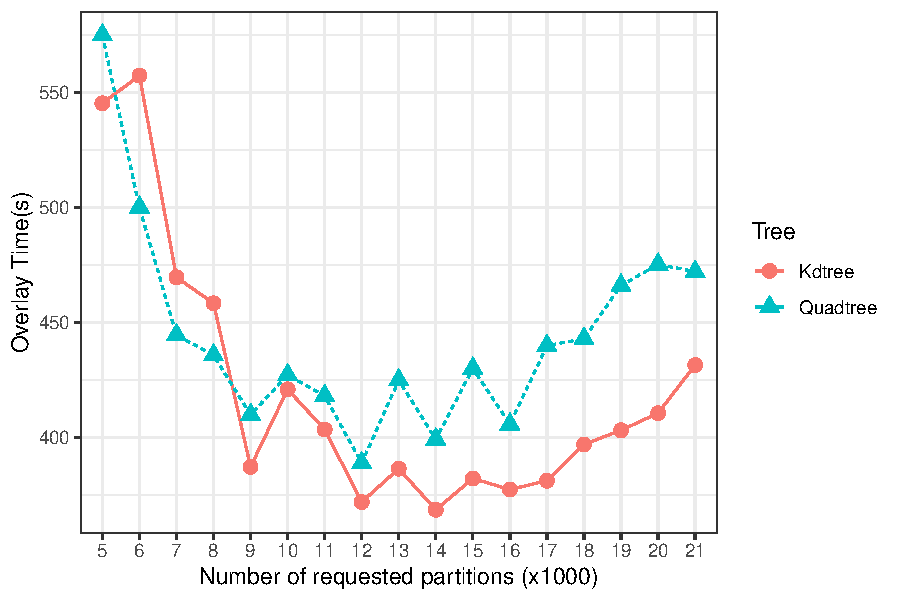
\includegraphics[width=0.49\linewidth]{chapterSDCEL/K_Overlay_GADM.pdf} \\
%         (a) & (b)
%     \end{tabular}
%     \caption{Execution time for the overlay operation using a spatial data structure in the MainUS (a)and GADM (b) dataset.} \label{fig:k_overlay_us}
% \end{figure}

%Once the data is assigned to their partitions, the overlay operation can be executed.  Figure \ref{fig:k_overlay_us} shows the overlay performance under each partition strategy, for different number of cells. The Kd-tree approach performs better; as the quadtree tends to generate more and emptier cells, its performance is directly affected.

%As it was said before, in particular on partitioning based on Kdtree, the smaller number of cells/partitions used in this approach give also an improvement on the impact of shuffling during the partition strategy because the number and size of the resulting partitions have a lower impact into the communication cost.

%Finally, we consider the speed-up and scale-up performance using the kd-tree partitioning. Figure \ref{fig:k_scale_speed_us}(a) shows the speed-up performance using the MainUS dataset (36M edges) while varying the number of nodes (for 3, 6, and 12 nodes). Similar to the quadtree partitioning strategy, the kd-tree partitioning shows good speed-up performance. As resources duplicate the execution time improves almost by a half.

%Figure \ref{fig:k_scale_speed_us}(b) shows the scale-up performance of the kd-tree partitioning approach. We followed the same procedure described in Section \ref{sec:speed_scale} to generate datasets for 8M, 16M, and 32M edges from the MainUS dataset and ran the kd-tree partitioning strategy with 3, 6, and 12 nodes, respectively. Again the kd-tree partitioning shows good speed-up performance, which remains flat as the load per node is almost equal.

% \begin{figure}
%     \centering
%     \begin{tabular}{cc}
%         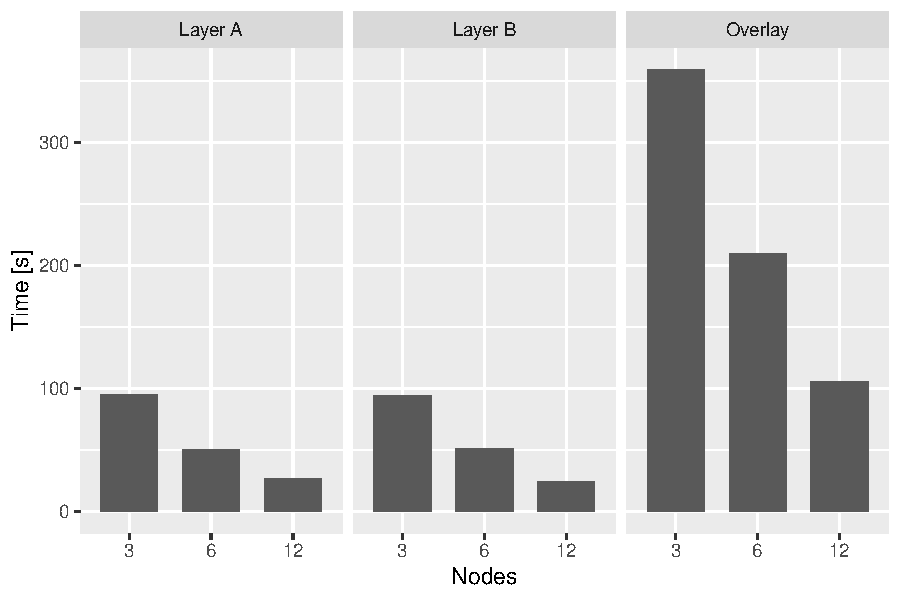
\includegraphics[width=0.49\linewidth]{chapterSDCEL/US_speedup.pdf} & 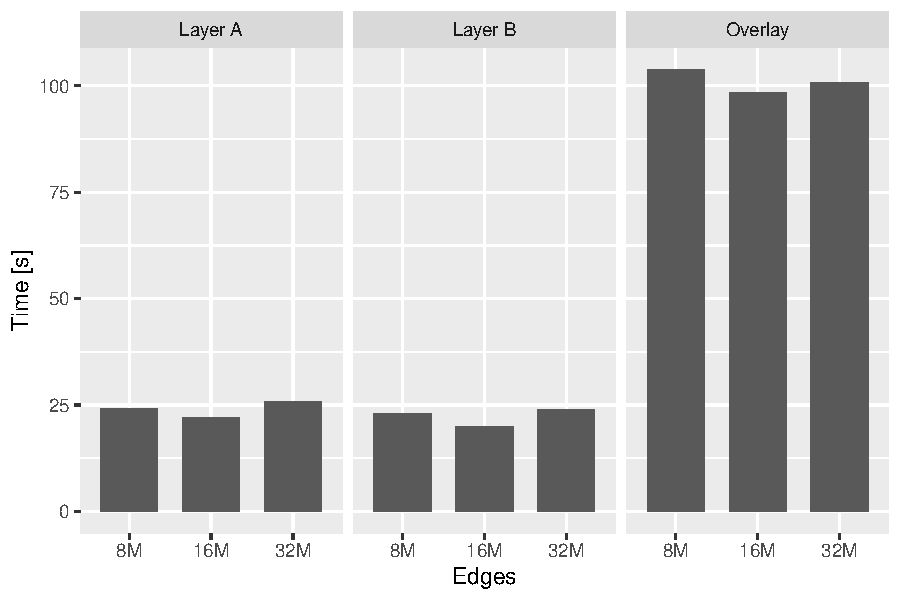
\includegraphics[width=0.49\linewidth]{chapterSDCEL/US_scaleup.pdf} \\
%         (a) & (b)
%     \end{tabular}
%     \caption{(a)Speed Up and (b) Scale Up performance of the Kdtree partitioning using the MainUS dataset.} \label{fig:k_scale_speed_us}
% \end{figure}


%% Extension
%\subsection{Polygonization Scalability}\label{sec:expr:query}
% \begin{table}
%     \centering
%     \caption{Polygonization Evaluation Dataset}
%     \label{table:polygonization:datasets}
%     \begin{tabular}{c c c c c}
%         \toprule
%         Dataset  & Area & Number of Line Segments & Faces \\
%         \midrule
%         USA & 9.83 $Mkm^2$ & 152$M$ & 5$M$ \\
%         South America & 17.8 $Mkm^2$ & 155$M$ & 7$M$\\
%         North America & 24.7 $Mkm^2$ & 240$M$ & 10$M$ \\
%         Africa & 30.4 $Mkm^2$ & 288$M$ & 10$M$  \\
%         Europe & 10.2 $Mkm^2$ & 563$M$ & 25$M$ \\
%         Asia & 44.6 $Mkm^2$ & 557$M$ & 23$M$ \\
%         \bottomrule
%     \end{tabular}
% \end{table}

% \begin{figure}
% \centering
% 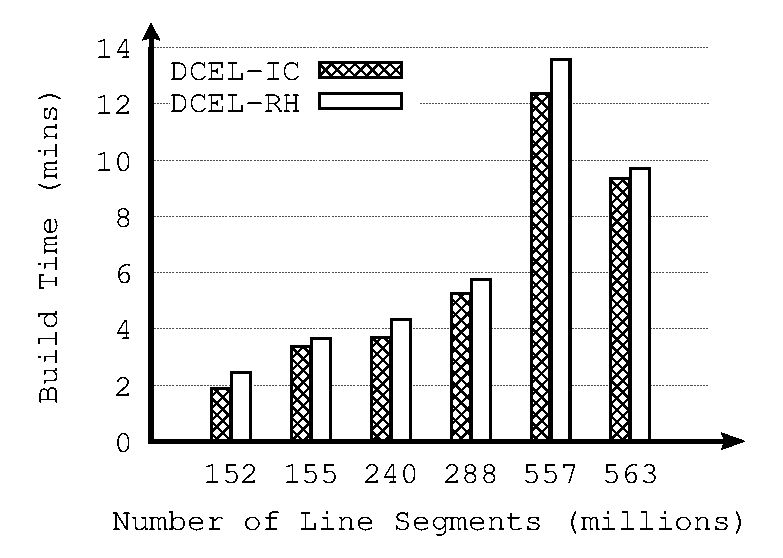
\includegraphics[width=0.48\linewidth]{chapterSDCEL/Experiments/n_records.eps}
% 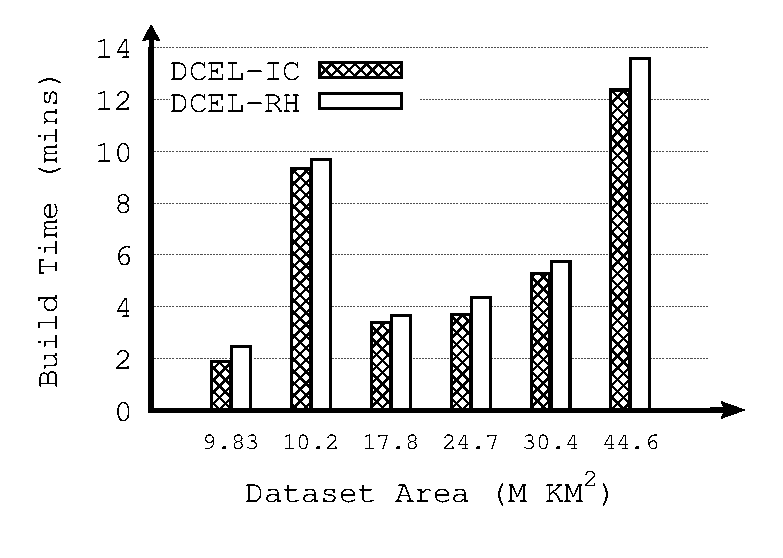
\includegraphics[width=0.48\linewidth]{chapterSDCEL/Experiments/area.eps}
% \caption{Polygonization Performance on Real Road Networks.}
% \label{fig:exp:query}
% \end{figure}

%Figure \ref{fig:exp:query} evaluates the scalability of the polygonization approach using the different evaluation datasets summarized in Table \ref{table:polygonization:datasets}.  We implemented our polygonization framework on Apache Sedona \cite{yu_spatial_2018}. The experiment is based on a Java 8  implementation and utilizes a Spark 2.3 cluster with two driver nodes and 12 worker nodes. All nodes run Linux CentOS 8.2 (64-bit). Each driver node is equipped with 128GB of RAM, while each worker node has 64GB of RAM. To increase parallelism, we divided the 12 worker nodes into 84 worker executors. Each executor is a separate JVM process with dedicated resources, such as memory and CPU cores. The distribution of these executors across the nodes is managed by the resource negotiator (YARN), which allocates resources for Spark jobs based on the availability of cores and memory. YARN typically balances resources across the cluster, so executors are likely to be evenly distributed, though some variation may occur due to resource availability at runtime. Assuming an even distribution, each worker node would run approximately 7 executors, as calculated by $\frac{84}{12} = 7$.

%As discussed in Section \ref{sec:rem}, the Rem Phase has two different approaches depending on the input data received from the Gen Phase. The first approach is to process the remaining half-edges iteratively, denoted as \textit{DCEL-RH}. In comparison, the second approach processes the incomplete cycles generated from the first phase iteratively denoted as \textit{DCEL-IC}.

%From Figure \ref{fig:exp:query}, we draw three conclusions; (1) first, the cardinality of the input dataset has a positive correlation with the build time; as the number of line segments increases, the build time also increases, as shown in Figure \ref{fig:exp:query}(a). However, we see that we have close cardinality for Asia (557M) and Europe (563M) datasets, but there is a noticeable difference in the build time; moreover, the build time for the Europe dataset is less than that of the Asia dataset. This drives us to the second conclusion; (2) for datasets with close or similar cardinalities, the area of the dataset has a positive correlation with the build time shown in Figure \ref{fig:exp:query}(b). Hence the build time of the Europe dataset (10.2 $Mkm^2$) is less than that of the Asia dataset (44.6 $Mkm^2$), even though Europe has a slightly larger dataset.  (3) The third conclusion is that for all evaluated datasets, the \textit{DCEL-IC} beats \textit{DCEL-RH}.


%% Extension
%\subsection{Polygonization Speed Up Evaluation} \label{sec:expr:speedup}
% \begin{figure}[tb]
% 	\centering
% 	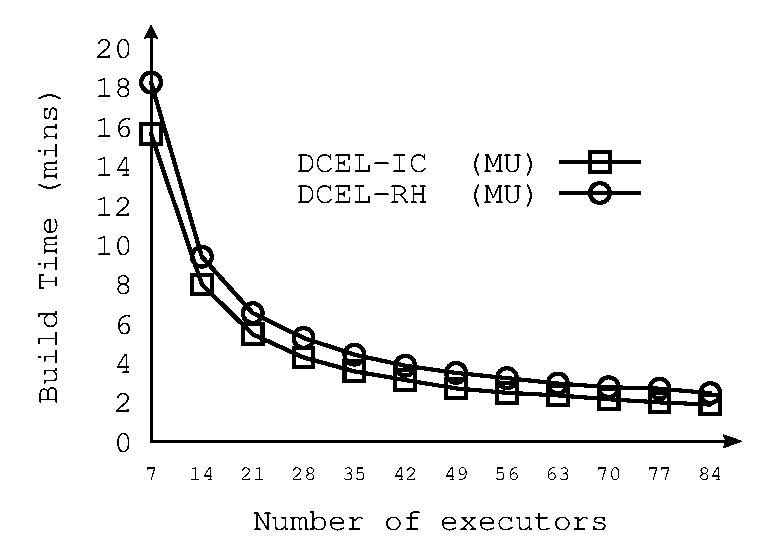
\includegraphics[width=8.8cm]{chapterSDCEL/Experiments/speedup.eps}
% 	\caption{Polygonization speed up evaluation using the USA dataset}
% 	\label{fig:exp:speedup}
% \end{figure}

%Figure \ref{fig:exp:speedup} shows the effect of increasing the number of executors on the build time for the USA dataset.  At each step in the figure, we add 7 more executors, which is approximately equivalent to adding one additional node.  Overall, our approach has good speedup performance. As the number of executors is doubled from 7 executors to 14 executors, the build time is almost halved.  This trend goes on as we double the number of executors. As we increase the number of executors from 7 to 84, the build time is decreased by a factor of 8.


%% Extension
%\subsection{Overlaying Polygons with Dangle and Cut Edges}
% \begin{table}
%     \caption{Overlaying Polygons with Dangle and Cut Edges Dataset}
%     \label{tab:dangles}
%     \begin{tabular}{c c c c}
%         \toprule
%         Dataset & Number Layer $A$ of Polygons & Number of Layer $B$ Edges & Result Polygons \\
%         \midrule
%         TN & 1,272 & 3,380,780 & 41,761 \\
%         GA & 1,633 & 4,647,171 & 49,125 \\
%         NC & 1,272 & 7,212,604 & 22,413 \\
%         TX & 4,399  & 8,682,950 & 98,635 \\
%         VA & 1,554 & 8,977,361 & 38,941 \\
%         CA & 7,038 & 9,103,610 & 96,916\\
%         \bottomrule
%     \end{tabular}
% \end{table}

% \begin{figure}
%     \centering
%     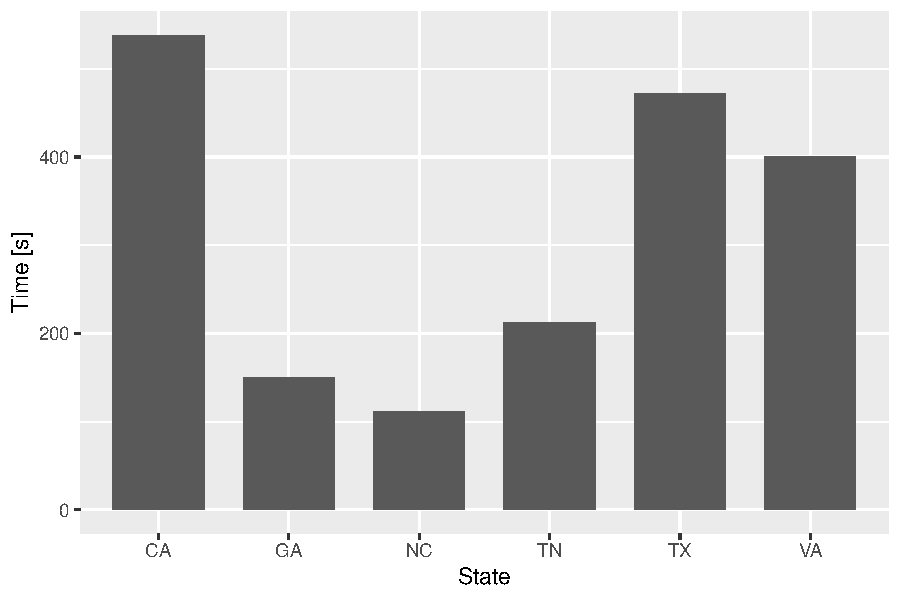
\includegraphics[width=0.7\linewidth]{chapterSDCEL/states.pdf}
%     \caption{Overlaying State polygons with dangle and cut edges.}
%     \label{fig:dangle}
% \end{figure}

%In this section, we examine the performance of overlaying polygons with dangle and cut edges resulting from the polygonization as detailed in Section \ref{sec:over_dang}.  Table \ref{tab:dangles} shows the number of polygons for each state for the first layer of the overlay. It also shows the number of dangle and cut edges per state for the second layer of the overlay. Finally, it shows the number of resultant polygons per state.  From Figure \ref{fig:dangle}, we conclude that the running time is affected by the number of dangle and cut edges and the number of intersections between the two layers (represented by the number of generated polygons).  TN and GA have a relatively smaller number of dangle and cut edges, so they have lower execution times compared to VA, TX, and CA. However, since the intersections in NC are significantly less than those of TN and GA, NC has the lowest execution time. TX, VA, and CA have a comparable number of edges; however, VA has the least number of intersections, resulting in lower execution time compared to TX and CA.

\chapter{Conclusions}
We introduced SDCEL, a scalable approach to compute the overlay operation among two layers that represent polygons from a planar subdivision of a surface. Both 
input layers use the DCEL edge-list data structure to store their polygons. Existing sequential DCEL overlay implementations fail for large datasets. We first 
presented a partition strategy which guarantees that each partition collects the required data from each layer to work independently. 
We also proposed several optimizations to improve performance. Our experimental evaluation using real datasets shows that SDCEL has very good scale-up and 
speed-up performance and can compute the overlay over very large layers (up to 37M edges) in few seconds.


\backmatter

\bmhead{Acknowledgements}
We would like to thank Sergio Rey from the Center for Geospatial Sciences for introducing us to the Scalable DCEL problem.

\section*{Declarations}

\begin{itemize}
\item Funding: This work was partially supported by the National Science Foundation under grants IIS-1901379, IIS-2237348, CNS-2031418, SES-1831615 and the Google-CAHSI research grant. 
\item Data availability: Data description and access is described in the experimental section.  The sources of the dataset are publicly available and the references and cited accordingly.
\end{itemize}


%%===========================================================================================%%
%% If you are submitting to one of the Nature Portfolio journals, using the eJP submission   %%
%% system, please include the references within the manuscript file itself. You may do this  %%
%% by copying the reference list from your .bbl file, paste it into the main manuscript .tex %%
%% file, and delete the associated \verb+\bibliography+ commands.                            %%
%%===========================================================================================%%

\bibliography{sdcel,ddcel-references}% common bib file
%% if required, the content of .bbl file can be included here once bbl is generated
%%\input sn-article.bbl

\end{document}
